\documentclass[12pt, a4paper]{article}

\usepackage[utf8x]{inputenc}
\usepackage[greek, english]{babel}
\usepackage{caption}
\usepackage[section]{placeins}
\usepackage{balance}
\usepackage{dblfloatfix}
\usepackage{hyperref}
\usepackage{color}
\usepackage{graphicx}
\usepackage{float}
\usepackage[margin=2cm]{geometry}
%\usepackage{graphicx,wrapfig,lipsum}

\newcommand{\en}{\selectlanguage{english}}
\newcommand{\gr}{\selectlanguage{greek}}

\hypersetup{
	colorlinks=true,
	linkcolor=blue,
	filecolor=magenta,
	urlcolor=blue,
}

\begin{document}
	
\gr
\begin{titlepage}
	
	\begin{center}
		\vspace*{0.5cm}
		
		\LARGE
		\textbf{\gr ΠΜΣ ΕΠΙΣΤΗΜΗ ΚΑΙ ΜΗΧΑΝΙΚΗ ΔΕΔΟΜΕΝΩΝ}
		
		\vspace{0.5cm}
		%\LARGE
		\Large 
		\gr{ΕΛΑΧΙΣΤΟΠΟΙΗΣΗ ΤΟΥ ΔΥΝΑΜΙΚΟΥ \en LENNARD-JONES \gr ΜΕ ΧΡΗΣΗ ΓΕΝΕΤΙΚΩΝ ΑΛΓΟΡΙΘΜΩΝ ΚΑΙ ΝΟΗΜΟΣΥΝΗΣ ΣΜΗΝΩΝ}
		
		\vspace{1.5cm}
		
		\textbf{Γεώργιος Βαρδάκας Α.Μ. 432}
		
		\vfill
		
\includegraphics[width=0.5\textwidth]{logo.png}
		
		\textbf{Υπεύθυνος Καθηγητής: \\Παρσόπουλος Κωνσταντίνος}
		\vfill
		
		%\bf{Τρίτη εργασία του μαθήματος της Βελτιστοποίησης Ακ.έτους 2020-2021}\\
		
		
		\vspace{0.8cm}
		
		\Large
		Τμήμα Μηχανικών Η/Υ και Πληροφορικής\\
		Πολυτεχνική Σχολή Πανεπιστημίου Ιωαννίνων\\
		%Ελλάδα\\
		\date{\today}
		
	\end{center}
\end{titlepage}


\tableofcontents
\newpage

\gr
\section{Εισαγωγή}

Με τον όρο συστάδες ατόμων \en(atom clusters) \gr χαρακτηρίζουμε τις ευσταθείς (συνήθως) ομάδες
ατόμων που σχηματίζονται διαμέσου φυσικών και χημικών δεσμών μεταξύ των ατόμων παράγοντας νέα στοιχεία. Οι φυσικές και χημικές ιδιότητες των συστάδων αλλάζουν σημαντικά σε σχέση με
τον αριθμό των ατόμων που τις απαρτίζουν. Οι ιδιότητες αυτές παίζουν πολύ σημαντικό ρόλο
στην κατασκευή νέων υλικών με συγκεκριμένα χαρακτηριστικά αγωγιμότητας, αποθήκευσης
ενέργειας κ.λ.π. \\

Μια από τις μεθόδους μελέτης ατομικών συστάδων έγκειται στη μελέτη του ενεργειακού προφίλ της συστάδας διαμέσου εξισώσεων δυναμικού \en (potential) \gr που περιγράφουν τις
αλληλεπιδράσεις μεταξύ των ατόμων. ΄Ενα τέτοιο μοντέλο συστάδων, το οποίο
αποδεικνύεται ιδιαίτερα ακριβές για την περίπτωση των αδρανών αερίων, είναι εκείνες των \en
Lennard-Jones (Lennard-Jones clusters). \gr
Η δομή αυτών των συστάδων, περιγράφει τη διάταξη των ατόμων στο χώρο επηρεάζουν άμεσα την ελάχιστη τιμή της δυναμικής ενέργειας του  συστήματος. \\

Η ελάχιστη τιμή της δυναμικής ενέργειας μιας τέτοιας συστάδας ατόμων συνήθως αντιστοιχεί στη θεμελιώδη κατάσταση του συστήματος κι επηρεάζεται άμεσα από τη δομή,
δηλαδή τη διάταξη των ατόμων της στον χώρο.\\

\textbf{Σκοπός της παρούσας εργασίας} είναι η εύρεση της βέλτιστης διάταξης των ατόμων στο χώρο με στόχο την εύρεση εκείνης της δομής που ελαχιστοποιεί τη δυναμική ενέργεια της συστάδας όπως έχουν ορίσει οι \en Lennard-Jones\gr. Η συνάρτηση δυναμικού \en Lennard-Jones \gr που υπολογίζει την δυναμική ενέργεια μιας συστάδας Ν ατόμων προκύπτει ως εξής:\\

Έστω ότι μια συστάδα $X$ αποτελείται από $N$ άτομα, $X = \{x_{1}, ..., x_{N}\}$ και κάθε $x_{i}$ ορίζει τις συντεταγμένες του στον χώρο ως $x_{i} = (x_{i1}, x_{i2}, x_{i3})^{T}$. Κατά συνέπεια ορίζεται ως $X = \{x_{11}, x_{12}, x_{13}, ..., x_{N1}, x_{N2}, x_{N3}\}$. Συμβολίζουμε ως $r_{ij} = ||x_{i} - x_{j} ||_{2}$ την Ευκλείδια απόσταση των ατόμων $x_{i}$ και $x_{j}$ για τα οποία η ενέργεια που προκύπτει για το ζεύγος αυτό δίνεται από την σχέση $u_{ij} = ( \frac{\sigma}{r_{ij}} )^{12} - ( \frac{\sigma}{r_{ij}} )^{6}$. Τέλος η δυναμική ενέργεια ολόκληρης της συστάδας των N ατόμων, που καλούμαστε να ελαχιστοποιήσουμε, δίνεται από τη συνάρτηση δυναμικού \en Lennard-Jones\gr: $E_{LJ} = 4\epsilon\sum\limits_{i=1}^{N-1}\sum\limits_{j=i+1}^{N} u_{ij}$, όπου $\sigma$ \en(equilibrium pair separation) \gr και $\epsilon$ \en(pair well depth) \gr είναι παράμετροι του δυναμικού. Η παρούσα εργασία θα επικεντρωθεί σε συστάδες με παραμέτρους $\sigma = \epsilon = 1$.

\section{Εξελικτικοί αλγόριθμοι και νοημοσύνη σμηνών}

Οι αλγόριθμοι που θα εξεταστούν ανήκουν στην γενική κατηγορία των μεθόδων βελτιστοποίησης χωρίς παραγώγους και συγκεκριμένα στην κατηγορία των εξελικτικών αλγορίθμων και νοημοσύνης σμηνών. Πιο συγκεκριμένα οι μεθοδολογίες που εξετάστηκαν είναι οι εξής:

\begin{itemize}
	\item Γενετικός αλγόριθμος δυαδικής αναπαράστασης με επιλογή \en roulette wheel. \gr
	\item Γενετικός αλγόριθμος δυαδικής αναπαράστασης με επιλογή \en tournament selection. \gr
	\item Γενετικός αλγόριθμος πραγματικής αναπαράστασης με επιλογή \en tournament selection. \gr
	\item Μέθοδος \en Particle Swarm Optimization \gr με \en global best \gr μοντέλο.
	\item Μέθοδος \en Particle Swarm Optimization \gr με \en local best \gr μοντέλο
\end{itemize}

\subsection{Γενετικός αλγόριθμος δυαδικής αναπαράστασης}
\label{sub:GAB}
Ο τρόπος λειτουργίας των Γενετικών Αλγορίθμων είναι εμπνευσμένος από τη βιολογία. Χρησιμοποιεί την ιδέα της εξέλιξης ως φυσικής επιλογής, διασταύρωσης και γενετικής μετάλλαξης. Αρχικά, στην διαδικασία του Γενετικού Αλγορίθμου αρχικοποιείται ένα τυχαίο σύνολο πληθυσμού, συνήθως με τυχαίες τιμές, δημιουργώντας ένα αρχικό σύνολο λύσεων. Στην περίπτωση της δυαδικής αναπαράστασης ο πληθυσμός αυτός είναι αρχικοποιημένος με τιμές 0 ή 1. Έπειτα ο πληθυσμός από δυαδική αναπαράσταση μετατρέπεται σε πραγματική (\en decoding\gr), έτσι ώστε κάθε μέλος του πληθυσμού να αξιολογηθεί με βάση την συναρτησιακή του τιμή. Στη συνέχεια παρατίθεται το κύριο μέρος του αλγορίθμου που καλείται επαναληπτικά με τους εξής κεντρικούς άξονες: \\

\textbf{Επιλογή:} είναι το πρώτο βήμα του γενετικού αλγορίθμου, όπου από τον πληθυσμό επιλέγονται με βάση την συναρτησιακή τους τιμή τα καλύτερα υποψήφια μέλη του. Οι δύο μέθοδοι της επιλογής που εξετάστηκαν στην εργασία είναι η επιλογή με \en roulette wheel \gr καθώς και με \en tournament selection. \\

\gr Στην επιλογή με \en roulette wheel \gr αναθέτουμε σε όλα τα μέλη του πληθυσμού ένα \en fitness score \gr με βάση την θέση που κατέχει το κάθε μέλος λαμβάνοντας υπόψιν τη συναρτησιακή του τιμή (εφόσον οι συναρτησιακές τιμές είναι ταξινομημένες σε φθίνουσα σειρά). Στην συνέχεια το \en fitness score \gr του μέλους $p_{i}$ υπολογίζεται ως εξής: $\phi_{i} = 2 - s + 2(s - 1) \frac{\rho_{i} - 1}{N - 1}, i = 1, ...,N$, όπου $\rho_{i}$ η θέση του μέλους $p_{i}$ και $s$ παράμετρος επιλεκτικής πίεσης ($s \in [1, 2]$). Στην συνέχεια κάνοντας χρήση των \en fitness score \gr του πληθυσμού υπολογίζουμε τις πιθανότητες επιλογής του κάθε μέλους κανονικοποιώντας τα \en fitness score\gr. Έπειτα δειγματολειπτούμε ομοιόμορφα κάνοντας χρήση της ομοιόμορφης κατανομής N τυχαίους αριθμούς στο διάστημα $[0, 1]$ όπου και επιλέγονται μέλη των οποίων οι τυχαίοι αριθμοί βρίσκονται κατανεμημένοι εντός των εκάστωτε διαστημάτων πιθανότητας.\\

Στην επιλογή με \en tournament selection \gr σημαντικό ρόλο παίζει η παράμετρος που ονομάζεται μέγεθος τουρνουά (\en tournament size\gr). Το μέγεθος τουρνουά λαμβάνει τιμές από [1, Ν]. Με την διαδικασία αυτή επιλέγονται τυχαία μέλη από τον πληθυσμό, όσα και το μέγεθος του τουρνουά σε πλήθος, και διαλέγουμε αυτόν με την καλύτερη συναρτησιακή τιμή. Αυτή η διαδικασία επαναλαμβάνεται Ν φορές.\\

\textbf{Διασταύρωση:} αποτελεί το δεύτερο βήμα του γενετικού αλγορίθμου, όπου από τον επιλεγμένο πληθυσμό διαλέγονται με κάποια πιθανότητα (\en crossover rate\gr) μέλη με σκοπό να κάνουν απογόνους. Στην συνέχεια το \en "DNA" \gr των γονέων διαχωρίζεται σε ένα πλήθος σημείων (\en crossover points\gr) τα οποία συνιστούν δυο ακόμη μέλη που ονομάζουμε απογόνους (παιδιά). Οι απόγονοι λαμβάνουν εναλλάξ κομμάτια \en "DNA" \gr από τους δύο γονείς τους. Στο τέλος της διαδικασίας οι απόγονοι αντικαθιστούν τους γονείς στον πληθυσμό. \\


\textbf{Μετάλλαξη:} συνιστά το τελευταίο βασικό βήμα του γενετικού αλγορίθμου, όπου από τον διασταυρωμένο πληθυσμό επιλέγονται με κάποια πιθανότητα συνιστώσες μελών (\en mutation rate\gr) για μετάλλαξη. Στην διαδικασία αυτή η  αρχική τιμή των υπο μετάλλαξη συνιστωσών αλλάζει/μεταβάλλεται από $i\rightarrow j \quad i,j=0,1$, δηλαδή εάν έχουν τιμή 1 γίνονται 0 και αντίστροφα.\\

Τέλος ανάμεσα στον αρχικό πληθυσμό και στον υπό μετάλλαξη πληθυσμό διαλέγονται οι N καλύτεροι με βάση την συναρτησιακή τους τιμή ώς αρχική τιμή πληθυσμού για την επόμενη επανάληψη.

\begin{table}[h]
	\centering
	\begin{tabular}{ | c || c | }
		\hline
		\en Parameter & \en Value \\ 
		
		\hline
		\en Population size & 1000 \\ 
		
		\hline
		\en Selective pressure & 1.3 \\
		
		\hline
		\en Tournament size & 100\\  
		
		\hline
		\en Crossover rate & 0.5\\
		
		\hline
		\en Crossover points & 6\\ 
		
		\hline
		\en Mutation rate & 0.1\\  
		
		\hline
		\en $\epsilon$ & $10^{-3}$\\  
		\hline
	
	\end{tabular}
	\caption{Τιμές παραμέτρων του γενετικού αλγορίθμου δυαδικής αναπαράστασης}
	\label{tab:GAB_Par}
\end{table}


\subsection{Γενετικός αλγόριθμος πραγματικής αναπαράστασης}
Οι αρχές λειτουργίας αυτής της μεθόδου είναι ίδιες με αυτές που περιγράφηκαν στην προηγούμενη \hyperref[sub:GAB]{παράγραφο}. Η κύρια διαφορά της είναι ότι η συγκεκριμένη μέθοδος ακολουθεί πραγματική και όχι δυαδική αναπαράσταση και δεν απαιτείται η διαδικασία του \en decoding\gr. Πλέον ο πληθυσμός αρχικοποιείται τυχαία με πραγματικές τιμές και αξιολογείται με βάση τις συναρτησιακές τους τιμές δημιουργώντας το αρχικό σύνολο λύσεων. Όπως και στην προηγούμενη μέθοδο οι βασικές διαδικασίες είναι η επιλογή, η διασταύρωση και η μετάλλαξη. Η διαδικασία της επιλογής είναι ακριβώς η ίδια με εκείνη που περιγράφηκε παραπάνω.\\

\textbf{Πραγματική Διασταύρωση:} αποτελεί το δεύτερο βήμα του γενετικού αλγορίθμου με πραγματική αναπαράσταση, όπου από τον επιλεγμένο πληθυσμό διαλέγονται με κάποια πιθανότητα (\en crossover rate\gr) μέλη του ώστε να να δημιουργήσουν απογόνους. Στην συνέχεια το \en "DNA" \gr των γονέων συνδυάζεται με την παρακάτω διαδικασία για την δημιουργία ενός απογόνου: Έστω $o = (o_{1}, ..., o_{n})$ απόγονος του $p_{i1}, p_{i2}$, τότε η συνιστώσα $o_{j} = r_{j}p_{i1,j} + (1-r_{j})p_{i2}$ με $r_{j}\sim U(-\delta, 1 + \delta)$ τυχαίος αριθμός με $\delta > 0$. \\

\textbf{Πραγματική Μετάλλαξη:} συνιστά το τελευταίο βασικό βήμα του γενετικού αλγορίθμου με πραγματική αναπαράσταση, όπου από τον διασταυρωμένο πληθυσμό επιλέγονται με κάποια πιθανότητα συνιστώσες μελών (\en mutation rate\gr) για να υποστούν μετάλλαξη. Στην διαδικασία αυτή στις υπό μετάλλαξη συνιστώσες, προστίθεται ένας τυχαίο αριθμός $z \sim N(0, \sigma^{2})$, όπου το $3\sigma$ είναι ίσο με το πλησιέστερο (άνω ή κάτω) όριο του χώρου αναζήτησης, ούτως ώστε μόνο ένα πολύ μικρό ποσοστό της τάξης του $0.03\%$ των επιλεγμένων προς μετάλλαξη συνιστωσών να αποκλίνει ελάχιστα εκτός του χώρου αναζήτησης.\\

Τέλος ανάμεσα στον αρχικό πληθυσμό και σε εκείνον που προκύπτει μετά το πέρας της μετάλλαξης πληθυσμό επιλέγονται από το δείγμα οι Ν καλύτεροι με βάση την συναρτησιακή τους τιμή ώς αρχική τιμή συνόλου πληθυσμού για την επόμενη επανάληψη.

\begin{table}[h]
	\centering
	\begin{tabular}{ | c || c | }
		\hline
		\en Parameter & \en Value \\ 
		
		\hline
		\en Population size & 1000 \\ 
		
		\hline
		\en Tournament size & 100\\  
		
		\hline
		\en Crossover rate & 0.5\\
		
		\hline
		\en Mutation rate & 0.1\\  
		
		\hline
		\en $\delta$ & 0.25\\  
		
		\hline
		
	\end{tabular}
	\caption{Τιμές παραμέτρων του γενετικού αλγορίθμου πραγματικής αναπαράστασης}
	\label{tab:GAR_Par}
\end{table}

\subsection{\en Particle Swarm Optimization\gr}

Ο τρόπος λειτουργίας της νοημοσύνης σμηνών (\en PSO\gr) είναι εμπνευσμένος από τη συλλογική συμπεριφορά μη κατανεμημένων, αυτοοργανωμένων φυσικών συστημάτων. Η νοημοσύνη σμήνους είναι μια ιδιότητα των συστημάτων που επιδεικνύουν συλλογικά ευφύη συμπεριφορά. Αρχικά, στην διαδικασία της μεθόδου \en Particle Swarm Optimization \gr  αρχικοποιείται τυχαία ένα σμήνος δημιουργώντας το αρχικό σύνολο λύσεων καθώς και μία αρχική τυχαία ταχύτητα για κάθε μέλος του σμήνους. Επίσης για το κάθε μέλος του σμήνους υπάρχει η καλύτερη θέση που έχει επισκεφθεί καθώς και η γειτονιά του η οποία και καθορίζει με ποια άλλα σωματίδια θα ανταλλάξει πληροφορία. Πρακτικά κάθε γειτονιά αποτελείται από ένα πλήθος δεικτών άλλων σωματιδίων με τα οποία ανταλλάσεται η πληροφορία καλύτερης θέσης. Οι διάφορες τοπολογίες των γειτονιών των σωματιδίων κατασκευάζουν και διαφορετικά μοντέλα του αλγορίθμου. Τα μοντέλα που μελετήθηκαν στην εργασία είναι το μεντέλο \en global best \gr και \en local best\gr. Στο μοντέλο \en global best \gr το κάθε σωματίδιο ανταλλάσει πληροφορία με όλα τα υπόλοιπα του πληθυσμού. Στην περίπτωση του \en local best \gr μοντέλου το \en i-\grσωματίδιο ανταλλάσει πληροφορία μόνο με τα σωματίδια με δείκτες $i-\rho, ..., \rho+i$ όπου $\rho$ είναι η ακτίνα της γειτονίας. Τελικά το σμήνος αξιολογείται με βάση την συναρτησιακή του τιμή και ακολουθεί το κύριο μέρος του αλγορίθμου που καλείται επαναληπτικά. \\

\textbf{Υπολογισμός ταχύτητας:} σε αυτή τη διαδικασία, υπολογίζεται η καινούργια ταχύτητα του κάθε σωματιδίου του σμήνους με βάση τον τύπο: 
\begin{center}
	$v_{ij}^{t+1} = \chi [v_{ij}^{t} + rand()c_{1}(p_{ij}^{t} - x_{ij}^{t}) + rand()c_{2}(p_{g_{i}j}^{t} - x_{ij}^{t})]$
\end{center}
όπου $g_{i}$ δείκτης του καλύτερου σωματιδίου στην γειτονιά συγκεκριμένης ακτίνας, $\chi,c_{1}, c_{2}$ θετικοί παράμετροι και $rand()$ τυχαίοι αριθμοί στο διάστημα [0, 1].\\

\textbf{Έλεγχος ταχύτητας:} σε αυτό το βήμα ελέγχεται εάν η ταχύτητα έχει ξεπεράσει κάποια μέγιστη τιμή (καθορίζεται από την παράμετρο \en alpha\gr), έτσι ώστε να μειωθεί στο μέγιστο δυνατό όριο της. Η διαδικασία αυτή γίνεται προληπτικά για να μην έχουμε φαινόμενα έκρηξης του σμήνους. Κύριο στόχο έχει να αποτρέψει τα σωματίδια να αναπτύξουν τόσο μεγάλες ταχύτητες που θα τα φέρουν εκτός του χώρου αναζήτησης.\\

\textbf{Υπολογισμός θέσης:} σε αυτό το βήμα υπολογίζουμε τις καινούργιες θέσεις του σμήνους με βάση τη σχέση: $x_{ij}^{t+1} = x_{ij}^{t} + v_{ij}^{t+1}$, μεταβάλλοντας τα δηλαδή κατ' αυτό το τρόπο στον χώρο αναζήτησης.\\

\textbf{Έλεγχος σμήνους:} στο βήμα αυτό ελέγχεται εάν τα μέλη του σμήνους έχουν βγει εκτός του χώρου αναζήτησης. Εάν κάποιο μέλος έχει ξεφύγει τότε τοποθετείται στο όριο του χώρου αναζήτησης.\\

Τέλος οι καινούργιες λύσεις αξιολογούνται με βάση την συναρτησιακή τους τιμή και πραγματοποιείται η ανανέωση των καλύτερων θέσεων του πληθυσμού έως την συγκεκριμένη χρονική στιγμή.

\begin{table}[h]
	\centering
	\begin{tabular}{ | c || c | }
		\hline
		\en Parameter & \en Value \\ 
		
		\hline
		\en Swarm size & 1000 \\ 
		
		\hline
		\en local best $\rho$ & 5\\
		
		\hline
		\en global best $\rho$ & 500\\
		
		\hline
		\en Alpha & 0.5\\
		
		\hline
		\en $c_{1}$ & 2.05\\
		
		\hline
		\en $c_{2}$ & 2.05\\
		
		\hline
		\en $\chi$ & 0.729\\
		
		\hline
		
	\end{tabular}
	\caption{Τιμές παραμέτρων της \en PSO\gr}
	\label{tab:PSO_Par}
\end{table}

\section{Πειράματα}
Στην τρέχουσα ενότητα παρατίθενται τα αποτελέσματα των πειραμάτων για τα διαφορετικά πλήθη ατόμων $N$. Για κάθε πείραμα το επιτρεπτό πλήθος συναρτησιακών υπολογισμών προσδιορίζεται από την σχέση  \underline{$Τ = Ν \times 10^{5} $}  και $N$ το πλήθος των ατόμων. Σε όλα τα πειράματα έχει πραγματοποιηθεί το στατιστικό τεστ \underline{\en Wilcoxon \gr}  με επίπεδο σημαντικότητας \underline{$a = 0.05$}. Σαν πρωτεύον κριτήριο χρησιμοποιήθηκε η ποιότητα της λύσης των μεθόδων και σαν δευτερεύον κριτήριο η ταχύτητα εντοπισμού της λύσης. Στα αποτελέσματα οι μέθοδοι του Γενετικού Αλγορίθμου συμβολίζονται ώς \en GA \gr ενώ ακολοθεί αντίστοιχα  το \en Binary/Real \gr στην περίπτωση δυαδικής ή πραγματικής αναπαράστασης καθώς και το \en rw/t \gr για τις μεθόδους επιλογής \en roulette wheel/tournament \gr αντίστοιχα. Επίσης η \en Particle Swarm Optimization \gr συμβολίζεται ως \en PSO \gr και ακολουθεί το είδος του μοντέλου ως \en gbest/lbest\gr. Οι πίνακες στατιστικών των μεθόδων έχουν στρογγυλοποιηθεί στο τρίτο δεκαδικό ψηφίο. 


\subsection{Αποτελέσματα για πλήθος ατόμων $N = 4$}
Στο \hyperref[box:sol_qual_N4]{\en boxplot \gr} που ακολουθεί παρατίθενται οι λύσεις των μεθόδων για τα 30 πειράματα που πραγματοποιήθηκαν. Είναι εμφανές ότι η μέθοδος του γενετικού αλγορίθμου με πραγματική αναπαράσταση καθώς και οι μέθοδοι \en PSO \gr πέτυχαν τα καλύτερα αποτελέσματα καθώς στην μέση περίπτωση (\hyperref[tab:sol_qual_N4]{πίνακας}) βρέθηκε το ολικό ελάχιστο της συνάρτησης, σύμφωνα με τους πίνακες της επίσημης \href{http://doye.chem.ox.ac.uk/jon/structures/LJ/tables.150.html}{σελίδας}. Αυτό πρακτικά σημαίνει ότι βρέθηκε η δομή των ατόμων που ελαχιστοποιούν το δυναμικό \en Lennard-Jones\gr.
 
Στην συνέχεια πραγματοποιήθηκε στατιστικός έλεγχος με τεστ \en Wilcoxon \gr ώστε να διαπιστωθεί εάν οι κατανομές των δειγμάτων των λύσεων έχουν στατιστικά σημαντική διαφορά μεταξύ τους. Τα αποτελέσματα δείχνουν ότι όλες οι μέθοδοι έχουν στατιστικά σημαντική διαφορά μεταξύ τους (\hyperref[tab:sol_qual_pval_N4]{πίνακας}), ωστόσο είναι τόσο μικρή που δεν είναι αντιληπτή λόγω στρογγυλοποίησης των αποτελεσμάτων τους στους αντίστοιχους πίνακες. 

Σαν δεύτερο κριτήριο έχει χρησιμοποιηθεί η ταχύτητα εύρεσης της λύσης. Εκ των τριών καλύτερων μεθόδων ταχύτερη είναι η \en PSO \gr με μοντέλο το \en global best \gr (\hyperref[tab:iter_N4]{πίνακας}). Η διαφορά τους είναι στατιστικά σημαντική συγκρινόμενη με την άλλη εκδοχή της \en PSO \gr αλλά όχι με τον γενετικό αλγόριθμο  (\hyperref[tab:iter_pval_N4]{πίνακας}). Με βάση τα αποτελέσματα οδηγούμαστε στο συμπέρασμα  ότι η καλύτερη μέθοδος για την επίλυση του συγκεκριμένου προβλήματος είναι η \en PSO \gr με μοντέλο \en global best\gr, ως πιο γρήγορη, καθώς οι δειγματοληπτικές μέσες τιμές και των τριών έχουν πετύχει το ολικό ελάχιστο.

\begin{figure}[H]
	\centering
	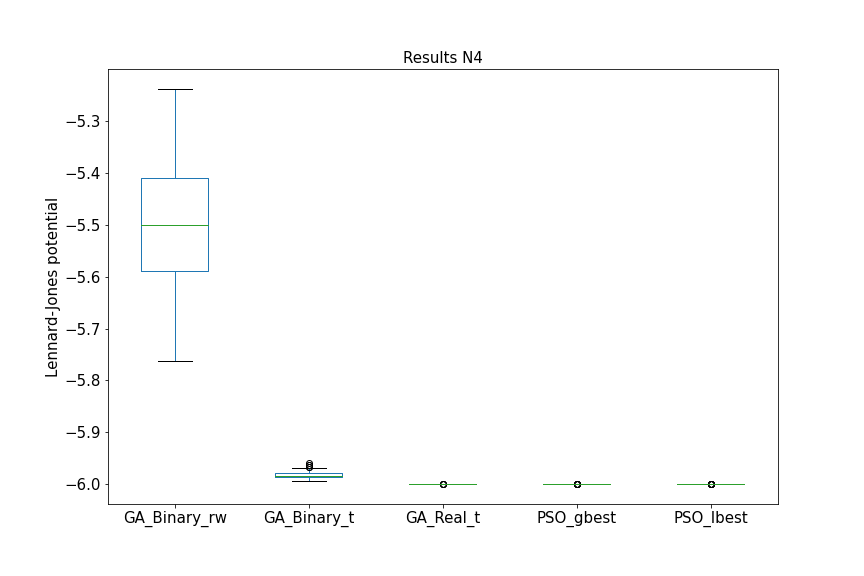
\includegraphics[width=0.85\textwidth, height=0.4\textheight]{../Results/N4/Boxplot_solutions_quality.png}
	
	\caption{\en Boxplot \gr λύσεων των μεθόδων για $N = 4$.}
	\label{box:sol_qual_N4}
\end{figure}

\begin{table}[H]
	\centering
	\begin{tabular}{| c | c | c | c | c | c |}
		
		\hline
		\en Method & \en Mean & \en Median & \en St.Dev. & \en Min & \en Max \\
		
		\hline
		\en GA\_Binary\_rw & -5.496 & -5.5 & 0.144 & -5.762 & -5.238 \\ 
		
		\hline
		\en GA\_Binary\_t & -5.981 & -5.983 & 0.009 & -5.994 & -5.96 \\ 
		
		\hline
		\en GA\_Real\_t & -6 & -6 & 0 & -6 & -5.999 \\ 
		
		\hline
		\en PSO\_gbest &  -6 & -6 & 0 & -6 & -5.999 \\ 
		
		\hline
		\en PSO\_lbest & -6 & -6 & 0 & -6 & -5.999 \\ 
		
		\hline
		
	\end{tabular}
	\caption{Στατιστικά λύσεων των μεθόδων για $N = 4$.}
	\label{tab:sol_qual_N4}
\end{table}

\begin{table}[H]
	\centering
	\begin{tabular}{| c | c | c | c | c | c |}
		
		\hline
		\en  & \en GAB\_rw & \en GAB\_t & \en GAR\_t & \en PSO\_gbest & \en PSO\_lbest\\
		
		\hline
		\en GAB\_rw & - & $1.73\mathrm{e}{-6}$ & $1.73\mathrm{e}{-6}$ & $1.73\mathrm{e}{-6}$ & $1.73\mathrm{e}{-6}$ \\ 
		
		\hline
		\en GAB\_t & - & - & $1.73\mathrm{e}{-6}$ & $1.73\mathrm{e}{-6}$ & $1.73\mathrm{e}{-6}$ \\ 
	
		\hline
		\en GAR\_t & - & - & - & $1.73\mathrm{e}{-6}$ & $1.89\mathrm{e}{-4}$ \\ 
		
		\hline
		\en PSO\_gbest & - & - & - & - & $2.84\mathrm{e}{-5}$\\ 
		
		\hline
		
	\end{tabular}
	\caption{\en Wilcoxon Test Pvalues \gr με κριτήριο τις ποιότητες των λύσεων για $N = 4$.}
	\label{tab:sol_qual_pval_N4}
\end{table}

\begin{table}[H]
	\centering
	\begin{tabular}{| c | c | c | c | c | c |}
		
		\hline
		\en Method & \en Mean & \en Median & \en St.Dev. & \en Min & \en Max \\
		
		\hline
		\en GA\_Binary\_rw & 291566 & 307000 & 79236 & 98000 & 396000 \\ 
		
		\hline
		\en GA\_Binary\_t & 303333 & 309000 & 67882 & 77000 & 400000 \\ 
		
		\hline
		\en GA\_Real\_t & 341366 & 367500 & 67098 & 87000 & 400000 \\ 
		
		\hline
		\en PSO\_gbest &  318766 & 310000 & 53339 & 218000 & 400000\\ 
		
		\hline
		\en PSO\_lbest & 397533 & 399000 & 3234 & 390000 & 400000 \\ 
		
		\hline
		
	\end{tabular}
	\caption{Στατιστικά της ταχύτητας εύρεσης των λύσεων για $N = 4$.}
	\label{tab:iter_N4}
\end{table}

\begin{table}[H]
	\centering
	\begin{tabular}{| c | c | c | c | c | c |}
		
		\hline
		\en  & \en GAB\_rw & \en GAB\_t & \en GAR\_t & \en PSO\_gbest & \en PSO\_lbest\\
		
		\hline
		\en GAB\_rw & - & 0.688 & 0.018 & 0.171 & $1.73\mathrm{e}{-6}$ \\ 
		
		\hline
		\en GAB\_t & - & - & 0.015 & 0.443 & $2.1\mathrm{e}{-6}$ \\ 
		
		\hline
		\en GAR\_t & - & - & - & 0.0999 & $1\mathrm{e}{-5}$ \\ 
		
		\hline
		\en PSO\_gbest & - & - & - & - & $4.2\mathrm{e}{-6}$\\ 
		
		\hline
		
	\end{tabular}
	\caption{\en Wilcoxon's Test Pvalues \gr με κριτήριο την ταχύτητας εύρεσης των λύσεων για $N = 4$.}
	\label{tab:iter_pval_N4}
\end{table}

\subsection{Αποτελέσματα για πλήθος ατόμων $N = 5$}
Στο \hyperref[box:sol_qual_N5]{\en boxplot\gr} που ακολουθεί παραθέτονται οι λύσεις των μεθόδων για τα 30 πειράματα που πραγματοποιήθηκαν. Ο γενετικός αλγόριθμος με πραγματική αναπαράσταση καθώς και η μέθοδος \en PSO \gr με μοντέλο \en local best \gr πέτυχαν τα καλύτερα αποτελέσματα καθώς στην μέση περίπτωση (\hyperref[tab:sol_qual_N5]{πίνακας}) βρήκαν το ολικό ελάχιστο της συνάρτησης καθώς και οι διακυμάνσεις τους είναι σχεδόν μηδενικές.

Ακολουθεί ο στατιστικός έλεγχος με τεστ \en Wilcoxon \gr στις κατανομές των δειγμάτων των λύσεων στον \hyperref[tab:sol_qual_pval_N5]{πίνακα}. Ο γενετικός αλγόριθμος με πραγματική αναπαράσταση και με την μέθοδο \en PSO local best \gr έχει στατιστικά σημαντικές διαφορές καθώς το $pvalue = 1.92\mathrm{e}{-6}$. Εκ των δύο η καλύτερη θεωρείται αυτή του γενετικού αλγορίθμου καθώς έχει τη χαμηλότερη μέση τιμή και τη μικρότερη διακύμανση στα αποτελέσματα της.

Σαν δεύτερο κριτήριο έχει χρησιμοποιηθεί η ταχύτητα εύρεσης της λύσης. Εκ των δύο καλύτερων μεθόδων ταχύτερη είναι ο γενετικός αλγόριθμος (\hyperref[tab:iter_N5]{πίνακας}). Ωστόσο η διαφορά τους δεν είναι στατιστικά σημαντική (\hyperref[tab:iter_pval_N5]{πίνακας}). Με βάση τα αποτελέσματα οδηγούμαστε στο συμπέρασμα  ότι η καλύτερη μέθοδος για το συγκεκριμένο πρόβλημα είναι ο γενετικός αλγόριθμος με πραγματική αναπαράσταση.


\begin{figure}[H]
	\centering
	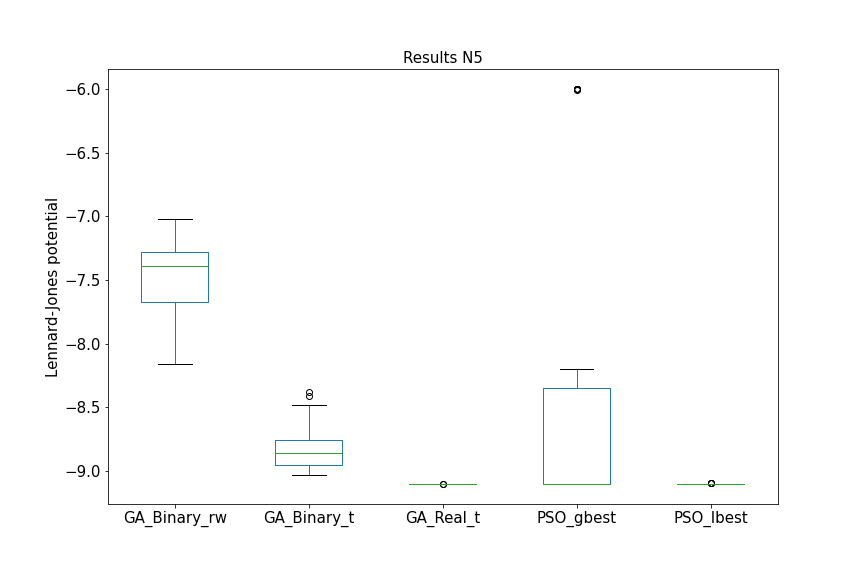
\includegraphics[width=0.85\textwidth, height=0.4\textheight]{../Results/N5/Boxplot_solutions_quality.png}
	
	\caption{\en Boxplot \gr λύσεων των μεθόδων για $N = 5$.}
	\label{box:sol_qual_N5}
\end{figure}

\begin{table}[H]
	\centering
	\begin{tabular}{| c | c | c | c | c | c |}
		
		\hline
		\en Method & \en Mean & \en Median & \en St.Dev. & \en Min & \en Max \\
		
		\hline
		\en GA\_Binary\_rw & -7.472 & -7.392 & 0.282 & -8.160 & -7.019 \\ 
		
		\hline
		\en GA\_Binary\_t & -8.821 & -8.860 & 0.176 & -9.032 & -8.376 \\ 
		
		\hline
		\en GA\_Real\_t & -9.104 & -9.104 & 0 & -9.104 & -9.104 \\ 
		
		\hline
		\en PSO\_gbest &  -8.409 & -9.104 & 1.245 & -9.105 & -6 \\ 
		
		\hline
		\en PSO\_lbest & -9.102 & -9.103 & 0.003 & -9.104 & -9.092\\ 
		
		\hline
		
	\end{tabular}
	\caption{Στατιστικά των λύσεων για $N = 5$.}
	\label{tab:sol_qual_N5}
\end{table}

\begin{table}[H]
	\centering
	\begin{tabular}{| c | c | c | c | c | c |}
		
		\hline
		\en  & \en GAB\_rw & \en GAB\_t & \en GAR\_t & \en PSO\_gbest & \en PSO\_lbest\\
		
		\hline
		\en GAB\_rw & - & $1.73\mathrm{e}{-6}$ & $1.28\mathrm{e}{-3}$ & $1.73\mathrm{e}{-6}$ & $1.73\mathrm{e}{-6}$ \\ 
		
		\hline
		\en GAB\_t & - & - & $1.73\mathrm{e}{-6}$ & $0.91$ & $1.73\mathrm{e}{-6}$ \\ 
		
		\hline
		\en GAR\_t & - & - & - & $0.033$ & $1.92\mathrm{e}{-6}$ \\ 
		
		\hline
		\en PSO\_gbest & - & - & - & - & $0.339$\\ 
		
		\hline
		
	\end{tabular}
	\caption{\en Wilcoxon's Test Pvalues \gr με κριτήριο τις ποιότητες των λύσεων για $N = 5$.}
	\label{tab:sol_qual_pval_N5}
\end{table}

\begin{table}[H]
	\centering
	\begin{tabular}{| c | c | c | c | c | c |}
		
		\hline
		\en Method & \en Mean & \en Median & \en St.Dev. & \en Min & \en Max \\
		
		\hline
		\en GA\_Binary\_rw & 379533 & 405000 & 97052 & 160000 & 496000 \\ 
		
		\hline
		\en GA\_Binary\_t & 420900 & 437000 & 59776 & 300000 & 498000 \\ 
		
		\hline
		\en GA\_Real\_t & 488166 & 498500 & 19138 & 429000 & 500000 \\ 
		
		\hline
		\en PSO\_gbest & 494466 & 500000 & 22335 & 381000 & 500000\\ 
		
		\hline
		\en PSO\_lbest & 497500 & 499000 & 2933 & 491000 & 500000 \\ 
		
		\hline
		
	\end{tabular}
	\caption{Στατιστικά της ταχύτητας εύρεσης των λύσεων για $N = 5$.}
	\label{tab:iter_N5}
\end{table}


\begin{table}[H]
	\centering
	\begin{tabular}{| c | c | c | c | c | c |}
		
		\hline
		\en  & \en GAB\_rw & \en GAB\_t & \en GAR\_t & \en PSO\_gbest & \en PSO\_lbest\\
		
		\hline
		\en GAB\_rw & - & 0.128 &  $5.7\mathrm{e}{-6}$ &  $1.1\mathrm{e}{-5}$ & $2\mathrm{e}{-6}$ \\ 
		
		\hline
		\en GAB\_t & - & - & $1.24\mathrm{e}{-5}$ & $5.74\mathrm{e}{-6}$ & $1.73\mathrm{e}{-6}$ \\ 
		
		\hline
		\en GAR\_t & - & - & - & 0.014 & 0.094 \\ 
		
		\hline
		\en PSO\_gbest & - & - & - & - & 0.039\\ 
		
		\hline
		
	\end{tabular}
	\caption{\en Wilcoxon's Test Pvalues \gr με κριτήριο την ταχύτητας εύρεσης των λύσεων για $N = 5$.}
	\label{tab:iter_pval_N5}
\end{table}

\subsection{Αποτελέσματα για πλήθος ατόμων $N = 6$}
Στο \hyperref[box:sol_qual_N6]{\en boxplot \gr} που ακολουθεί παρατίθενται οι λύσεις των μεθόδων για τα 30 πειράματα που πραγματοποιήθηκαν. Ο γενετικός αλγόριθμος με πραγματική αναπαράσταση καθώς και η μέθοδος \en PSO \gr με μοντέλο \en local best \gr πέτυχαν τα καλύτερα αποτελέσματα καθώς στην μέση περίπτωση (\hyperref[tab:sol_qual_N6]{πίνακας}) βρήκαν το ολικό ελάχιστο της συνάρτησης και οι διακυμάνσεις τους είναι μικρότερες των υπόλοιπων μεθόδων.

Ακολουθεί ο στατιστικός έλεγχος με τεστ \en Wilcoxon \gr στις κατανομές των δειγμάτων των λύσεων στον \hyperref[tab:sol_qual_pval_N6]{πίνακα}. Ο γενετικός αλγόριθμος με πραγματική αναπαράσταση και με την μέθοδο \en PSO local best \gr δεν έχουν στατιστικά σημαντική διαφορά καθώς το $pvalue = 0.245$. Εκ των δύο η καλύτερη θεωρείται αυτή του γενετικού αλγορίθμου καθώς έχει τη χαμηλότερη μέση τιμή και τη μικρότερη διακύμανση στα αποτελέσματα της.

Σαν δεύτερο κριτήριο έχει χρησιμοποιηθεί η ταχύτητα εύρεσης της λύσης. Εκ των δύο καλύτερων μεθόδων ταχύτερη είναι ο γενετικός αλγόριθμος (\hyperref[tab:iter_N6]{πίνακας}). Ωστόσο η διαφορά τους δεν είναι στατιστικά σημαντική (\hyperref[tab:iter_pval_N6]{πίνακας}). Με βάση τα ανωτέρω οδηγούμαστε στο συμπέρασμα ότι η καλύτερη μέθοδος για το συγκεκριμένο πρόβλημα είναι ο γενετικός αλγόριθμος με πραγματική αναπαράσταση.


\begin{figure}[H]
	\centering
	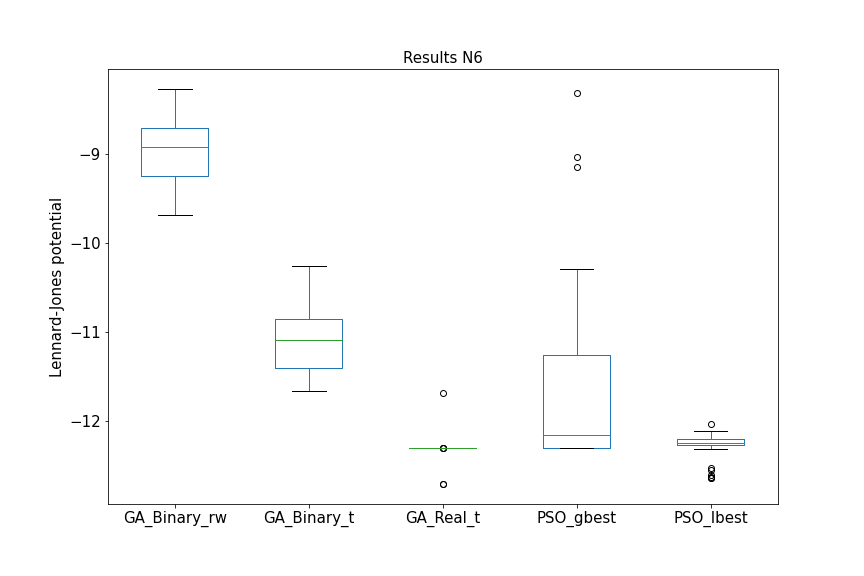
\includegraphics[width=0.85\textwidth, height=0.4\textheight]{../Results/N6/Boxplot_solutions_quality.png}
	
	\caption{\en Boxplot \gr λύσεων των μεθόδων για $N = 6$.}
	\label{box:sol_qual_N6}
\end{figure}


\begin{table}[H]
	\centering
	\begin{tabular}{| c | c | c | c | c | c |}
		
		\hline
		\en Method & \en Mean & \en Median & \en St.Dev. & \en Min & \en Max \\
		
		\hline
		\en GA\_Binary\_rw & -8.945 & -8.922 & 0.396 & -9.687 & -8.263 \\ 
		
		\hline
		\en GA\_Binary\_t & -11.062 & -11.088 & 0.391 & -11.659 & -10.259 \\ 
		
		\hline
		\en GA\_Real\_t & -12.31 & -12.303 & 0.156 & -12.712 & -11.691 \\ 
		
		\hline
		\en PSO\_gbest &  -11.537 & -12.162 & 1.110 & -12.303 & -8.313\\ 
		
		\hline
		\en PSO\_lbest & -12.292 & -12.245 & 0.169 & -12.648 & -12.037\\ 
		
		\hline
		
	\end{tabular}
	\caption{Στατιστικά των λύσεων για $N = 6$.}
	\label{tab:sol_qual_N6}
\end{table}

\begin{table}[H]
	\centering
	\begin{tabular}{| c | c | c | c | c | c |}
		
		\hline
		\en  & \en GAB\_rw & \en GAB\_t & \en GAR\_t & \en PSO\_gbest & \en PSO\_lbest\\
		
		\hline
		\en GAB\_rw & - & $1.73\mathrm{e}{-6}$ & $1.73\mathrm{e}{-6}$ & $2.13\mathrm{e}{-6}$ & $1.73\mathrm{e}{-6}$ \\ 
		
		\hline
		\en GAB\_t & - & - & $1.73\mathrm{e}{-6}$ & $0.018$ & $1.73\mathrm{e}{-6}$ \\ 
		
		\hline
		\en GAR\_t & - & - & - & $1\mathrm{e}{-5}$ & $0.245$ \\ 
		
		\hline
		\en PSO\_gbest & - & - & - & - & $3.9\mathrm{e}{-4}$\\ 
		
		\hline
		
	\end{tabular}
	\caption{\en Wilcoxon's Test Pvalues \gr με κριτήριο τις ποιότητες των λύσεων για $N = 6$.}
	\label{tab:sol_qual_pval_N6}
\end{table}


\begin{table}[H]
	\centering
	\begin{tabular}{| c | c | c | c | c | c |}
		
		\hline
		\en Method & \en Mean & \en Median & \en St.Dev. & \en Min & \en Max \\
		
		\hline
		\en GA\_Binary\_rw & 434700 & 464500 & 127806 & 85000 & 593000 \\ 
		
		\hline
		\en GA\_Binary\_t & 511266 & 532000 & 75092 & 297000 & 598000 \\ 
		
		\hline
		\en GA\_Real\_t & 593866 & 600000 & 16336 & 541000 & 600000 \\ 
		
		\hline
		\en PSO\_gbest & 599466 & 600000 & 2556 & 586000 & 600000\\ 
		
		\hline
		\en PSO\_lbest & 598266 & 600000 & 2923 & 589000 & 600000 \\ 
		
		\hline
		
	\end{tabular}
	\caption{Στατιστικά της ταχύτητας εύρεσης των λύσεων για $N = 6$.}
	\label{tab:iter_N6}
\end{table}

\begin{table}[H]
	\centering
	\begin{tabular}{| c | c | c | c | c | c |}
		
		\hline
		\en  & \en GAB\_rw & \en GAB\_t & \en GAR\_t & \en PSO\_gbest & \en PSO\_lbest\\
		
		\hline
		\en GAB\_rw & - & 0.018 &  $3.18\mathrm{e}{-6}$ &  $1.73\mathrm{e}{-6}$ & $1.73\mathrm{e}{-6}$ \\ 
		
		\hline
		\en GAB\_t & - & - & $6.33\mathrm{e}{-6}$ & $1.73\mathrm{e}{-6}$ & $1.92\mathrm{e}{-6}$ \\ 
		
		\hline
		\en GAR\_t & - & - & - & 0.092 & 0.732 \\ 
		
		\hline
		\en PSO\_gbest & - & - & - & - & 0.017\\ 
		
		\hline
		
	\end{tabular}
	\caption{\en Wilcoxon's Test Pvalues \gr με κριτήριο την ταχύτητας εύρεσης των λύσεων για $N = 6$.}
	\label{tab:iter_pval_N6}
\end{table}

\subsection{Αποτελέσματα για πλήθος ατόμων $N = 7$}
Στο \hyperref[box:sol_qual_N7]{\en boxplot \gr} που ακολουθεί παρατίθενται οι λύσεις των μεθόδων για τα 30 πειράματα που πραγματοποιήθηκαν. Ο γενετικός αλγόριθμος με πραγματική αναπαράσταση και με τη μέθοδο \en PSO \gr με μοντέλο \en local best \gr πέτυχαν τα καλύτερα αποτελέσματα καθώς είναι αυτές με την μικρότερη μέση τιμή (\hyperref[tab:sol_qual_N7]{πίνακας}) και επίσης βρίσκονται κοντά στο ολικό ελάχιστο. Ο γενετικός αλγόριθμος πραγματικής αναπαράστασης κατάφερε να πετύχει τον ολικό ελαχιστοποιητή της συνάρτησης τουλάχιστον μία φορα όπως βλέπουμε στην στήλη \en min \gr του στατιστικού πίνακα.

Ακολουθεί ο στατιστικός έλεγχος με τεστ \en Wilcoxon \gr στις κατανομές των δειγμάτων των λύσεων στον \hyperref[tab:sol_qual_pval_N7]{πίνακα}. Ο γενετικός αλγόριθμος με πραγματική αναπαράσταση και με τη μέθοδο \en PSO local best \gr έχουν στατιστικά σημαντική διαφορά καθώς το $pvalue = 1.11\mathrm{e}{-3}$. Εκ των δύο η βέλτιστη θεωρείται αυτή του γενετικού αλγορίθμου καθώς έχει μικρότερη μέση τιμή.

Σαν δεύτερο κριτήριο έχει χρησιμοποιηθεί η ταχύτητα εύρεσης της λύσης. Οι δύο μέθοδοι δεν έχουν στατιστικά σημαντικές διαφορές στην ταχύτητα τους. Με βάση τα παραπάνω οδηγούμαστε στο συμπέρασμα ότι η καλύτερη μέθοδος για το συγκεκριμένο πρόβλημα είναι ο γενετικός αλγόριθμος με πραγματική αναπαράσταση.

Τα αποτελέσματα των πειραμάτων για πλήθος ατόμων με $Ν = 8, 9, 10, 15, 20$ είναι ίδια με αυτά αυτού του συγκεκριμένου πειράματος και για αυτό και  ως προς τη μέθοδο δεν τίθεται σκόπιμη η περαιτέρω ανάλυση τους. Η γραφική απεικόνιση των αποτελεσμάτων και η στατιστική ανάλυση παρατίθεται στις ενότητες που ακολουθούν.

\begin{figure}[H]
	\centering
	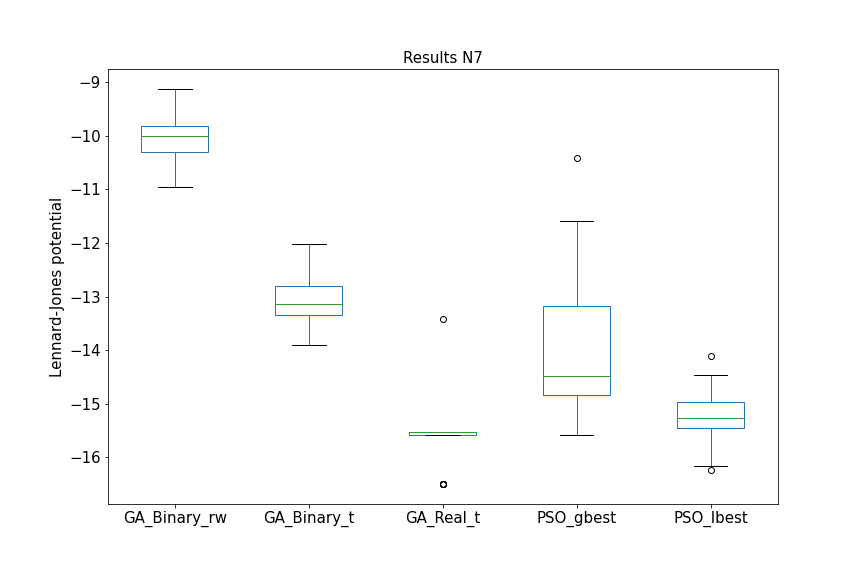
\includegraphics[width=0.85\textwidth, height=0.4\textheight]{../Results/N7/Boxplot_solutions_quality.png}
	
	\caption{\en Boxplot \gr λύσεων των μεθόδων για $N = 7$.}
	\label{box:sol_qual_N7}
\end{figure}


\begin{table}[H]
	\centering
	\begin{tabular}{| c | c | c | c | c | c |}
		
		\hline
		\en Method & \en Mean & \en Median & \en St.Dev. & \en Min & \en Max \\
		
		\hline
		\en GA\_Binary\_rw & -10.06 & -9.992 & 0.424 & -10.95 & -9.121 \\ 
		
		\hline
		\en GA\_Binary\_t & -13.056 & -13.133 & 0.47 & -13.912 & -12.019 \\ 
		
		\hline
		\en GA\_Real\_t & -15.665 & -15.533 & 0.577 & -16.505 & -13.415 \\ 
		
		\hline
		\en PSO\_gbest & -14.001 & -14.489 & 1.29 & -15.586 & -10.405\\ 
		
		\hline
		\en PSO\_lbest & -15.224 & -15.267 & 0.473 & -16.246 & -14.104\\ 
		
		\hline
		
	\end{tabular}
	\caption{Στατιστικά των λύσεων για $N = 7$.}
	\label{tab:sol_qual_N7}
\end{table}

\begin{table}[H]
	\centering
	\begin{tabular}{| c | c | c | c | c | c |}
		
		\hline
		\en  & \en GAB\_rw & \en GAB\_t & \en GAR\_t & \en PSO\_gbest & \en PSO\_lbest\\
		
		\hline
		\en GAB\_rw & - & $1.73\mathrm{e}{-6}$ & $1.73\mathrm{e}{-6}$ & $1.73\mathrm{e}{-6}$ & $1.73\mathrm{e}{-6}$ \\ 
		
		\hline
		\en GAB\_t & - & - & $1.92\mathrm{e}{-6}$ & $1.71\mathrm{e}{-3}$ & $1.73\mathrm{e}{-6}$ \\ 
		
		\hline
		\en GAR\_t & - & - & - & $1.73\mathrm{e}{-6}$ & $1.11\mathrm{e}{-3}$ \\ 
		
		\hline
		\en PSO\_gbest & - & - & - & - & $1.8\mathrm{e}{-5}$\\ 
		
		\hline
		
	\end{tabular}
	\caption{\en Wilcoxon's Test Pvalues \gr με κριτήριο τις ποιότητες των λύσεων για $N = 7$.}
	\label{tab:sol_qual_pval_N7}
\end{table}

\begin{table}[H]
	\centering
	\begin{tabular}{| c | c | c | c | c | c |}
		
		\hline
		\en Method & \en Mean & \en Median & \en St.Dev. & \en Min & \en Max \\
		
		\hline
		\en GA\_Binary\_rw & 448233 & 471000 & 171788 & 96000 & 685000 \\ 
		
		\hline
		\en GA\_Binary\_t & 521433 & 525000 & 116132 & 186000 & 694000 \\ 
		
		\hline
		\en GA\_Real\_t & 697600 & 700000 & 6483 & 674000 & 700000 \\ 
		
		\hline
		\en PSO\_gbest & 700000 & 700000 & 0 & 700000 & 700000\\ 
		
		\hline
		\en PSO\_lbest & 697200 & 698000 & 3652 & 687000 & 700000 \\ 
		
		\hline
		
	\end{tabular}
	\caption{Στατιστικά της ταχύτητας εύρεσης των λύσεων για $N = 7$.}
	\label{tab:iter_N7}
\end{table}

\begin{table}[H]
	\centering
	\begin{tabular}{| c | c | c | c | c | c |}
		
		\hline
		\en  & \en GAB\_rw & \en GAB\_t & \en GAR\_t & \en PSO\_gbest & \en PSO\_lbest\\
		
		\hline
		\en GAB\_rw & - & 0.066 & $1.73\mathrm{e}{-6}$ &  $1.73\mathrm{e}{-6}$ & $1.73\mathrm{e}{-6}$ \\ 
		
		\hline
		\en GAB\_t & - & - & $1.73\mathrm{e}{-6}$ & $1.73\mathrm{e}{-6}$ & $1.92\mathrm{e}{-6}$ \\ 
		
		\hline
		\en GAR\_t & - & - & - & 0.042 & 0.101 \\ 
		
		\hline
		\en PSO\_gbest & - & - & - & - & $8.27\mathrm{e}{-5}$\\ 
		
		\hline
		
	\end{tabular}
	\caption{\en Wilcoxon's Test Pvalues \gr με κριτήριο την ταχύτητας εύρεσης των λύσεων για $N = 7$.}
	\label{tab:iter_pval_N7}
\end{table}


\subsection{Αποτελέσματα για πλήθος ατόμων $N = 8$}

\begin{figure}[H]
	\centering
	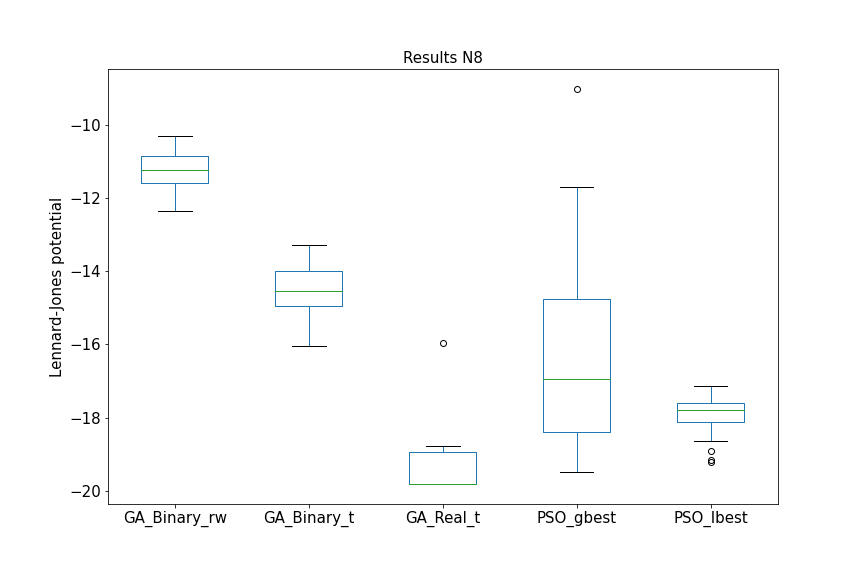
\includegraphics[width=0.85\textwidth, height=0.4\textheight]{../Results/N8/Boxplot_solutions_quality.png}
	
	\caption{\en Boxplot \gr λύσεων των μεθόδων για $N = 8$.}
	\label{box:sol_qual_N8}
\end{figure}

\begin{table}[H]
	\centering
	\begin{tabular}{| c | c | c | c | c | c |}
		
		\hline
		\en Method & \en Mean & \en Median & \en St.Dev. & \en Min & \en Max \\
		
		\hline
		\en GA\_Binary\_rw & -11.227 & -11.242 & 0.517 & -12.348 & -10.291 \\ 
		
		\hline
		\en GA\_Binary\_t & -14.456 & -14.532 & 0.722 & -16.028 & -13.27 \\ 
		
		\hline
		\en GA\_Real\_t & -19.4 & -19.821 & 0.785 & -19.821 & -15.954 \\ 
		
		\hline
		\en PSO\_gbest & -16.368 & -16.939 & 2.581 & -19.481 & -9.011\\ 
		
		\hline
		\en PSO\_lbest & -17.936 & -17.8 & 0.537 & -19.225 & -17.127\\ 
		
		\hline
		
	\end{tabular}
	\caption{Στατιστικά των λύσεων για $N = 8$.}
	\label{tab:sol_qual_N8}
\end{table}

\begin{table}[H]
	\centering
	\begin{tabular}{| c | c | c | c | c | c |}
		
		\hline
		\en  & \en GAB\_rw & \en GAB\_t & \en GAR\_t & \en PSO\_gbest & \en PSO\_lbest\\
		
		\hline
		\en GAB\_rw & - & $1.73\mathrm{e}{-6}$ & $1.73\mathrm{e}{-6}$ & $2.6\mathrm{e}{-6}$ & $1.73\mathrm{e}{-6}$ \\ 
		
		\hline
		\en GAB\_t & - & - & $1.73\mathrm{e}{-6}$ & $1.04\mathrm{e}{-3}$ & $1.73\mathrm{e}{-6}$ \\ 
		
		\hline
		\en GAR\_t & - & - & - & $5.75\mathrm{e}{-6}$ & $3.88\mathrm{e}{-6}$ \\ 
		
		\hline
		\en PSO\_gbest & - & - & - & - & $3.61\mathrm{e}{-3}$\\ 
		
		\hline
		
	\end{tabular}
	\caption{\en Wilcoxon's Test Pvalues \gr με κριτήριο τις ποιότητες των λύσεων για $N = 8$.}
	\label{tab:sol_qual_pval_N8}
\end{table}


\begin{table}[H]
	\centering
	\begin{tabular}{| c | c | c | c | c | c |}
		
		\hline
		\en Method & \en Mean & \en Median & \en St.Dev. & \en Min & \en Max \\
		
		\hline
		\en GA\_Binary\_rw & 515266 & 563500 & 208540 & 115000 & 772000 \\ 
		
		\hline
		\en GA\_Binary\_t & 603033 & 617500 & 129925 & 230000 & 794000 \\ 
		
		\hline
		\en GA\_Real\_t & 799033 & 800000 & 2697 & 788000 & 800000 \\ 
		
		\hline
		\en PSO\_gbest & 798000 & 800000 & 9273 & 749000 & 800000\\ 
		
		\hline
		\en PSO\_lbest & 798000 & 800000 & 3912 & 784000 & 800000 \\ 
		
		\hline
		
	\end{tabular}
	\caption{Στατιστικά της ταχύτητας εύρεσης των λύσεων για $N = 8$.}
	\label{tab:iter_N8}
\end{table}


\begin{table}[H]
	\centering
	\begin{tabular}{| c | c | c | c | c | c |}
		
		\hline
		\en  & \en GAB\_rw & \en GAB\_t & \en GAR\_t & \en PSO\_gbest & \en PSO\_lbest\\
		
		\hline
		\en GAB\_rw & - & 0.088 & $1.73\mathrm{e}{-6}$ &  $1.73\mathrm{e}{-6}$ & $1.73\mathrm{e}{-6}$ \\ 
		
		\hline
		\en GAB\_t & - & - & $1.73\mathrm{e}{-6}$ & $1.73\mathrm{e}{-6}$ & $1.73\mathrm{e}{-6}$ \\ 
		
		\hline
		\en GAR\_t & - & - & - & 0.661 & 0.185 \\ 
		
		\hline
		\en PSO\_gbest & - & - & - & - & 0.11 \\ 
		
		\hline
		
	\end{tabular}
	\caption{\en Wilcoxon's Test Pvalues \gr με κριτήριο την ταχύτητας εύρεσης των λύσεων για $N = 8$.}
	\label{tab:iter_pval_N8}
\end{table}


\subsection{Αποτελέσματα για πλήθος ατόμων $N = 9$}

\begin{figure}[H]
	\centering
	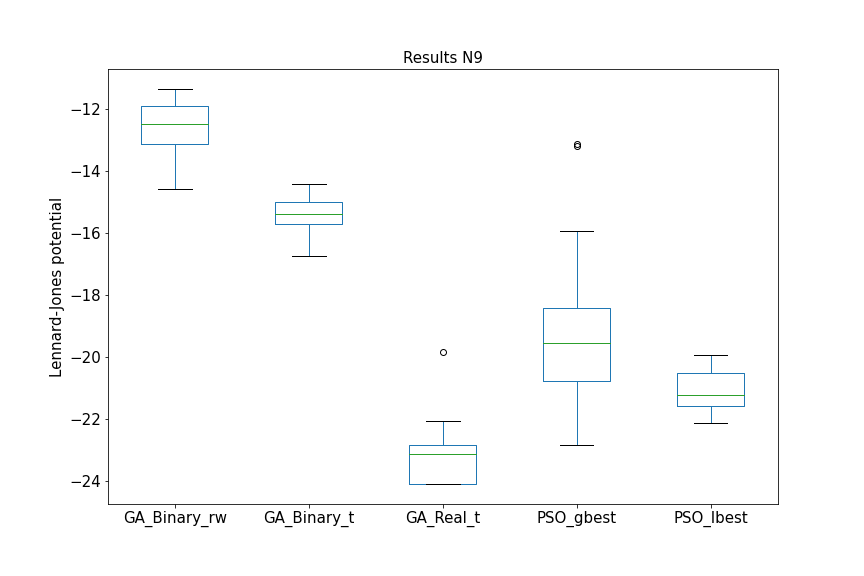
\includegraphics[width=0.85\textwidth, height=0.4\textheight]{../Results/N9/Boxplot_solutions_quality.png}
	
	\caption{\en Boxplot \gr λύσεων των μεθόδων για $N = 9$.}
	\label{box:sol_qual_N9}
\end{figure}

\begin{table}[H]
	\centering
	\begin{tabular}{| c | c | c | c | c | c |}
		
		\hline
		\en Method & \en Mean & \en Median & \en St.Dev. & \en Min & \en Max \\
		
		\hline
		\en GA\_Binary\_rw & -12.66 & -12.491 & 0.903 & -14.596 & -11.367 \\ 
		
		\hline
		\en GA\_Binary\_t & -15.464 & -15.397 & 0.6289 & -16.756 & -14.442 \\ 
		
		\hline
		\en GA\_Real\_t & -23.2067 & -23.134 & 0.98 & -24.113 & -19.847 \\ 
		
		\hline
		\en PSO\_gbest & -19.365 & -19.547 & 2.277 & -22.856 & -13.134\\ 
		
		\hline
		\en PSO\_lbest & -21.088 & -21.25 & 0.649 & -22.133 & -19.931\\ 
		
		\hline
		
	\end{tabular}
	\caption{Στατιστικά των λύσεων για $N = 9$.}
	\label{tab:sol_qual_N9}
\end{table}

\begin{table}[H]
	\centering
	\begin{tabular}{| c | c | c | c | c | c |}
		
		\hline
		\en  & \en GAB\_rw & \en GAB\_t & \en GAR\_t & \en PSO\_gbest & \en PSO\_lbest\\
		
		\hline
		\en GAB\_rw & - & $1.73\mathrm{e}{-6}$ & $1.73\mathrm{e}{-6}$ & $1.73\mathrm{e}{-6}$ & $1.73\mathrm{e}{-6}$ \\ 
		
		\hline
		\en GAB\_t & - & - & $1.73\mathrm{e}{-6}$ & $5.75\mathrm{e}{-6}$ & $1.73\mathrm{e}{-6}$ \\ 
		
		\hline
		\en GAR\_t & - & - & - & $3.52\mathrm{e}{-6}$ & $5.22\mathrm{e}{-6}$ \\ 
		
		\hline
		\en PSO\_gbest & - & - & - & - & $5.3\mathrm{e}{-4}$\\ 
		
		\hline
		
	\end{tabular}
	\caption{\en Wilcoxon's Test Pvalues \gr με κριτήριο τις ποιότητες των λύσεων για $N = 9$.}
	\label{tab:sol_qual_pval_N9}
\end{table}


\begin{table}[H]
	\centering
	\begin{tabular}{| c | c | c | c | c | c |}
		
		\hline
		\en Method & \en Mean & \en Median & \en St.Dev. & \en Min & \en Max \\
		
		\hline
		\en GA\_Binary\_rw & 662733 & 682000 & 153144 & 308000 & 880000 \\ 
		
		\hline
		\en GA\_Binary\_t & 700333 & 719500 & 124653 & 349000 & 900000 \\ 
		
		\hline
		\en GA\_Real\_t & 897533 & 900000 & 7181 & 864000 & 900000 \\ 
		
		\hline
		\en PSO\_gbest & 899933 & 900000 & 253 & 899000 & 900000\\ 
		
		\hline
		\en PSO\_lbest & 897900 & 899000 & 3835 & 885000 & 900000 \\ 
		
		\hline
		
	\end{tabular}
	\caption{Στατιστικά της ταχύτητας εύρεσης των λύσεων για $N = 9$.}
	\label{tab:iter_N9}
\end{table}


\begin{table}[H]
	\centering
	\begin{tabular}{| c | c | c | c | c | c |}
		
		\hline
		\en  & \en GAB\_rw & \en GAB\_t & \en GAR\_t & \en PSO\_gbest & \en PSO\_lbest\\
		
		\hline
		\en GAB\_rw & - & 0.465 & $1.73\mathrm{e}{-6}$ &  $1.73\mathrm{e}{-6}$ & $1.73\mathrm{e}{-6}$ \\ 
		
		\hline
		\en GAB\_t & - & - & $2.56\mathrm{e}{-6}$ & $2.56\mathrm{e}{-6}$ & $2.12\mathrm{e}{-6}$ \\ 
		
		\hline
		\en GAR\_t & - & - & - & 0.026 & 0.406 \\ 
		
		\hline
		\en PSO\_gbest & - & - & - & - & $5.5\mathrm{e}{-5}$\\ 
		
		\hline
		
	\end{tabular}
	\caption{\en Wilcoxon's Test Pvalues \gr με κριτήριο την ταχύτητας εύρεσης των λύσεων για $N = 9$.}
	\label{tab:iter_pval_N9}
\end{table}

\subsection{Αποτελέσματα για πλήθος ατόμων $N = 10$}

\begin{figure}[H]
	\centering
	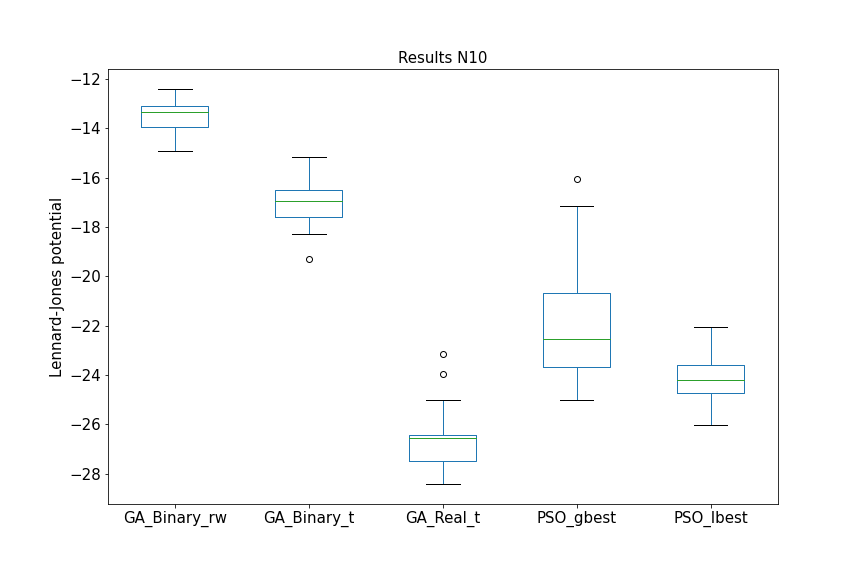
\includegraphics[width=0.85\textwidth, height=0.4\textheight]{../Results/N10/Boxplot_solutions_quality.png}
	
	\caption{\en Boxplot \gr λύσεων των μεθόδων για $N = 10$.}
	\label{box:sol_qual_N10}
\end{figure}

\begin{table}[H]
	\centering
	\begin{tabular}{| c | c | c | c | c | c |}
		
		\hline
		\en Method & \en Mean & \en Median & \en St.Dev. & \en Min & \en Max \\
		
		\hline
		\en GA\_Binary\_rw & -13.497 & -13.347 & 0.629 & -14.909 & -12.396 \\ 
		
		\hline
		\en GA\_Binary\_t & -17.033 & -16.933 & 0.885 & -19.274 & -15.17 \\ 
		
		\hline
		\en GA\_Real\_t & -26.531 & -26.558 & 1.127 & -28.422 & -23.163 \\ 
		
		\hline
		\en PSO\_gbest & -22.013 & -22.553 & 2.177 & -24.987 & -16.032\\ 
		
		\hline
		\en PSO\_lbest & -24.062 & -24.179 & 0.936 & -26.0126 & -22.0611\\ 
		
		\hline
		
	\end{tabular}
	\caption{Στατιστικά των λύσεων για $N = 10$.}
	\label{tab:sol_qual_N10}
\end{table}

\begin{table}[H]
	\centering
	\begin{tabular}{| c | c | c | c | c | c |}
		
		\hline
		\en  & \en GAB\_rw & \en GAB\_t & \en GAR\_t & \en PSO\_gbest & \en PSO\_lbest\\
		
		\hline
		\en GAB\_rw & - & $1.73\mathrm{e}{-6}$ & $1.73\mathrm{e}{-6}$ & $1.73\mathrm{e}{-6}$ & $1.73\mathrm{e}{-6}$ \\ 
		
		\hline
		\en GAB\_t & - & - & $1.73\mathrm{e}{-6}$ & $2.6\mathrm{e}{-6}$ & $1.73\mathrm{e}{-6}$ \\ 
		
		\hline
		\en GAR\_t & - & - & - & $1.92\mathrm{e}{-4}$ & $4.73\mathrm{e}{-6}$ \\ 
		
		\hline
		\en PSO\_gbest & - & - & - & - & $1.6\mathrm{e}{-4}$\\ 
		
		\hline
		
	\end{tabular}
	\caption{\en Wilcoxon's Test Pvalues \gr με κριτήριο τις ποιότητες των λύσεων για $N = 10$.}
	\label{tab:sol_qual_pval_N10}
\end{table}


\begin{table}[H]
	\centering
	\begin{tabular}{| c | c | c | c | c | c |}
		
		\hline
		\en Method & \en Mean & \en Median & \en St.Dev. & \en Min & \en Max \\
		
		\hline
		\en GA\_Binary\_rw & 682500 & 719000 & 247140 & 164000 & 996000 \\ 
		
		\hline
		\en GA\_Binary\_t & 718400 & 796000 & 235180 & 159000 & 987000 \\ 
		
		\hline
		\en GA\_Real\_t & 999266 & 1000000 & 2753 & 985000 & 1000000 \\ 
		
		\hline
		\en PSO\_gbest & 999966 & 1000000 & 182 & 999000 & 1000000\\ 
		
		\hline
		\en PSO\_lbest & 998700 & 999000 & 1235 & 996000 & 1000000 \\ 
		
		\hline
		
	\end{tabular}
	\caption{Στατιστικά της ταχύτητας εύρεσης των λύσεων για $N = 10$.}
	\label{tab:iter_N10}
\end{table}

\begin{table}[H]
	\centering
	\begin{tabular}{| c | c | c | c | c | c |}
		
		\hline
		\en  & \en GAB\_rw & \en GAB\_t & \en GAR\_t & \en PSO\_gbest & \en PSO\_lbest\\
		
		\hline
		\en GAB\_rw & - & 0.673 & $1.73\mathrm{e}{-6}$ &  $1.73\mathrm{e}{-6}$ & $1.73\mathrm{e}{-6}$ \\ 
		
		\hline
		\en GAB\_t & - & - & $1.73\mathrm{e}{-6}$ & $1.73\mathrm{e}{-6}$ & $1.73\mathrm{e}{-6}$ \\ 
		
		\hline
		\en GAR\_t & - & - & - & 0.047 & 0.007 \\ 
		
		\hline
		\en PSO\_gbest & - & - & - & - & $6.81\mathrm{e}{-5}$\\ 
		
		\hline
		
	\end{tabular}
	\caption{\en Wilcoxon's Test Pvalues \gr με κριτήριο την ταχύτητας εύρεσης των λύσεων για $N = 10$.}
	\label{tab:iter_pval_N10}
\end{table}

\subsection{Αποτελέσματα για πλήθος ατόμων $N = 15$}

\begin{figure}[H]
	\centering
	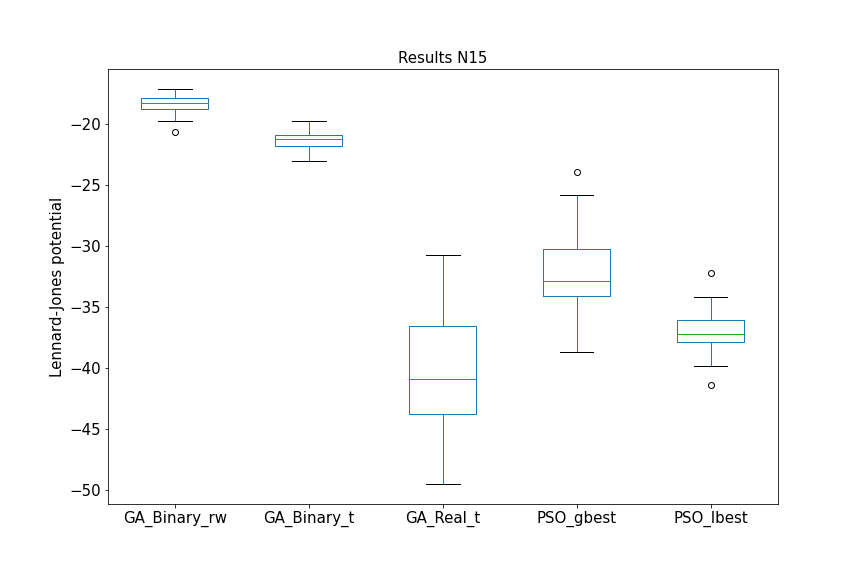
\includegraphics[width=0.85\textwidth, height=0.4\textheight]{../Results/N15/Boxplot_solutions_quality.png}
	
	\caption{\en Boxplot \gr λύσεων των μεθόδων για $N = 15$.}
	\label{box:sol_qual_N15}
\end{figure}

\begin{table}[H]
	\centering
	\begin{tabular}{| c | c | c | c | c | c |}
		
		\hline
		\en Method & \en Mean & \en Median & \en St.Dev. & \en Min & \en Max \\
		
		\hline
		\en GA\_Binary\_rw & -18.448 & -18.311 & 0.827 & -20.705 & -17.152 \\ 
		
		\hline
		\en GA\_Binary\_t & -21.406 & -21.247 & 0.766 & -23.102 & -19.802 \\ 
		
		\hline
		\en GA\_Real\_t & -40.3126 & -40.921 & 4.721 & -49.566 & -30.797 \\ 
		
		\hline
		\en PSO\_gbest & -32.123 & -32.871 & 3.389 & -38.747 & -23.979\\ 
		
		\hline
		\en PSO\_lbest & -37.002 & -37.2112 & 1.881 & -41.434 & -32.245\\ 
		
		\hline
		
	\end{tabular}
	\caption{Στατιστικά των λύσεων για $N = 15$.}
	\label{tab:sol_qual_N15}
\end{table}


\begin{table}[H]
	\centering
	\begin{tabular}{| c | c | c | c | c | c |}
		
		\hline
		\en  & \en GAB\_rw & \en GAB\_t & \en GAR\_t & \en PSO\_gbest & \en PSO\_lbest\\
		
		\hline
		\en GAB\_rw & - & $1.73\mathrm{e}{-6}$ & $1.73\mathrm{e}{-6}$ & $1.73\mathrm{e}{-6}$ & $1.73\mathrm{e}{-6}$ \\ 
		
		\hline
		\en GAB\_t & - & - & $1.73\mathrm{e}{-6}$ &  $1.73\mathrm{e}{-6}$ & $1.73\mathrm{e}{-6}$ \\ 
		
		\hline
		\en GAR\_t & - & - & - & $7.69\mathrm{e}{-6}$ & $1.83\mathrm{e}{-3}$ \\ 
		
		\hline
		\en PSO\_gbest & - & - & - & - & $2.88\mathrm{e}{-6}$\\ 
		
		\hline
		
	\end{tabular}
	\caption{\en Wilcoxon's Test Pvalues \gr με κριτήριο τις ποιότητες των λύσεων για $N = 15$.}
	\label{tab:sol_qual_pval_N15}
\end{table}


\begin{table}[H]
	\centering
	\begin{tabular}{| c | c | c | c | c | c |}
		
		\hline
		\en Method & \en Mean & \en Median & \en St.Dev. & \en Min & \en Max \\
		
		\hline
		\en GA\_Binary\_rw & 946733 & 999000 & 328535 & 140000 & 1401000 \\ 
		
		\hline
		\en GA\_Binary\_t & 916500 & 943500 & 311664 & 255000 & 1394000 \\ 
		
		\hline
		\en GA\_Real\_t & 1498300 & 1499000 & 3852 & 1479000 & 1500000 \\ 
		
		\hline
		\en PSO\_gbest & 1499933 & 1500000 & 253 & 1499000 & 1500000\\ 
		
		\hline
		\en PSO\_lbest & 1497800 & 1498500 & 2708 & 1491000 & 1500000 \\ 
		
		\hline
		
	\end{tabular}
	\caption{Στατιστικά της ταχύτητας εύρεσης των λύσεων για $N = 15$.}
	\label{tab:iter_N15}
\end{table}

\begin{table}[H]
	\centering
	\begin{tabular}{| c | c | c | c | c | c |}
		
		\hline
		\en  & \en GAB\_rw & \en GAB\_t & \en GAR\_t & \en PSO\_gbest & \en PSO\_lbest\\
		
		\hline
		\en GAB\_rw & - & 0.789 & $1.73\mathrm{e}{-6}$ &  $1.73\mathrm{e}{-6}$ & $1.73\mathrm{e}{-6}$ \\ 
		
		\hline
		\en GAB\_t & - & - & $1.73\mathrm{e}{-6}$ & $1.73\mathrm{e}{-6}$ & $1.73\mathrm{e}{-6}$ \\ 
		
		\hline
		\en GAR\_t & - & - & - & $5.67\mathrm{e}{-5}$ & 0.244 \\ 
		
		\hline
		\en PSO\_gbest & - & - & - & - & $1.7\mathrm{e}{-5}$\\ 
		
		\hline
		
	\end{tabular}
	\caption{\en Wilcoxon's Test Pvalues \gr με κριτήριο την ταχύτητας εύρεσης των λύσεων για $N = 15$.}
	\label{tab:iter_pval_N15}
\end{table}

\subsection{Αποτελέσματα για πλήθος ατόμων $N = 20$}

\begin{figure}[H]
	\centering
	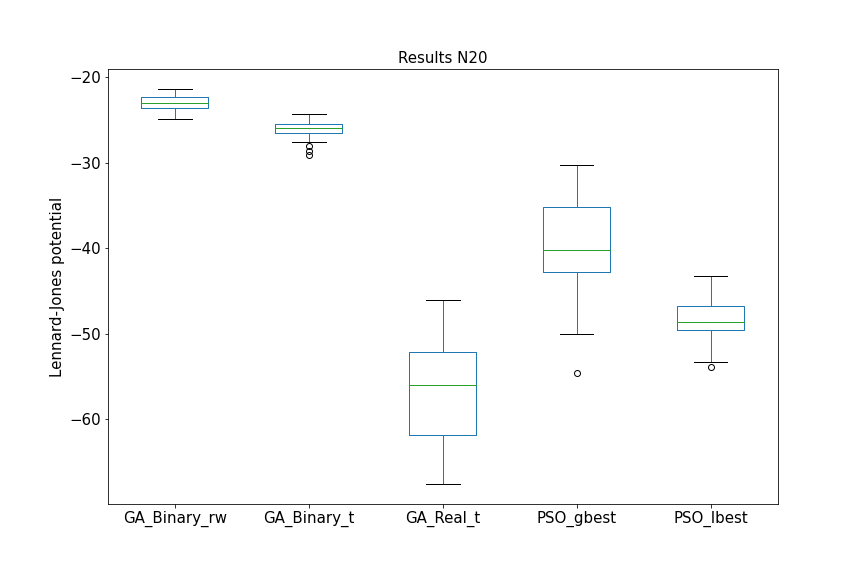
\includegraphics[width=0.85\textwidth, height=0.4\textheight]{../Results/N20/Boxplot_solutions_quality.png}
	
	\caption{\en Boxplot \gr λύσεων των μεθόδων για $N = 20$.}
	\label{box:sol_qual_N20}
\end{figure}

\begin{table}[H]
	\centering
	\begin{tabular}{| c | c | c | c | c | c |}
		
		\hline
		\en Method & \en Mean & \en Median & \en St.Dev. & \en Min & \en Max \\
		
		\hline
		\en GA\_Binary\_rw & -22.949 & -22.951 & 0.969 & -24.915 & -21.354 \\ 
		
		\hline
		\en GA\_Binary\_t & -26.116 & -25.96 & 1.101 & -29.046 & -24.245 \\ 
		
		\hline
		\en GA\_Real\_t & -56.759 & -55.992 & 5.780 & -67.595 & -46.007 \\ 
		
		\hline
		\en PSO\_gbest & -39.836 & -40.165 & 5.262 & -54.593 & -30.246\\ 
		
		\hline
		\en PSO\_lbest & -48.422 & -48.653 & 2.361 & -53.865 & -43.22\\ 
		\hline
		
	\end{tabular}
	\caption{Στατιστικά των λύσεων για $N = 20$.}
	\label{tab:sol_qual_N20}
\end{table}

\begin{table}[H]
	\centering
	\begin{tabular}{| c | c | c | c | c | c |}
		
		\hline
		\en  & \en GAB\_rw & \en GAB\_t & \en GAR\_t & \en PSO\_gbest & \en PSO\_lbest\\
		
		\hline
		\en GAB\_rw & - & $1.17\mathrm{e}{-6}$ & $1.17\mathrm{e}{-6}$ & $1.17\mathrm{e}{-6}$ & $1.17\mathrm{e}{-6}$ \\ 
		
		\hline
		\en GAB\_t & - & - & $1.17\mathrm{e}{-6}$ &  $1.17\mathrm{e}{-6}$ & $1.17\mathrm{e}{-6}$ \\ 
		
		\hline
		\en GAR\_t & - & - & - & $1.3\mathrm{e}{-6}$ & $2.82\mathrm{e}{-6}$ \\ 
		
		\hline
		\en PSO\_gbest & - & - & - & - & $5\mathrm{e}{-6}$\\ 
		
		\hline
		
	\end{tabular}
	\caption{\en Wilcoxon's Test Pvalues \gr με κριτήριο τις ποιότητες των λύσεων για $N = 20$.}
	\label{tab:sol_qual_pval_N20}
\end{table}

\begin{table}[H]
	\centering
	\begin{tabular}{| c | c | c | c | c | c |}
		
		\hline
		\en Method & \en Mean & \en Median & \en St.Dev. & \en Min & \en Max \\
		
		\hline
		\en GA\_Binary\_rw & 1289233 & 1348000 & 414877 & 527000 & 1912000 \\ 
		
		\hline
		\en GA\_Binary\_t & 1169500 & 1296500 & 478946 & 180000 & 1874000 \\ 
		
		\hline
		\en GA\_Real\_t & 1997166 & 1998500 & 3312 & 1988000 & 2000000 \\ 
		
		\hline
		\en PSO\_gbest & 1999766 & 2000000 & 504 & 1998000 & 2000000\\ 
		
		\hline
		\en PSO\_lbest & 1998433 & 1999000 & 2284 & 1990000 & 2000000 \\ 
		
		\hline
		
	\end{tabular}
	\caption{Στατιστικά της ταχύτητας εύρεσης των λύσεων για $N = 20$.}
	\label{tab:iter_N20}
\end{table}

\begin{table}[H]
	\centering
	\begin{tabular}{| c | c | c | c | c | c |}
		
		\hline
		\en  & \en GAB\_rw & \en GAB\_t & \en GAR\_t & \en PSO\_gbest & \en PSO\_lbest\\
		
		\hline
		\en GAB\_rw & - & 0.189 & $1.73\mathrm{e}{-6}$ &  $1.17\mathrm{e}{-6}$ & $1.17\mathrm{e}{-6}$ \\ 
		
		\hline
		\en GAB\_t & - & - & $1.17\mathrm{e}{-6}$ & $1.17\mathrm{e}{-6}$ & $1.17\mathrm{e}{-6}$ \\ 
		
		\hline
		\en GAR\_t & - & - & - & $9.91\mathrm{e}{-5}$ & 0.037 \\ 
		
		\hline
		\en PSO\_gbest & - & - & - & - & $6.7\mathrm{e}{-5}$\\ 
		
		\hline
		
	\end{tabular}
	\caption{\en Wilcoxon's Test Pvalues \gr με κριτήριο την ταχύτητας εύρεσης των λύσεων για $N = 20$.}
	\label{tab:iter_pval_N20}
\end{table}

\subsection{Συμπεράσματα}
Μετά την συγκεντρωτική ανάλυση των αποτελεσμάτων οδηγούμαστε στο συμπέρασμα ότι στο συγκεκριμένο πρόβλημα η καλύτερη μέθοδος είναι αυτή του γενετικού αλγορίθμου με πραγματική αναπαράσταση. Αυτό είναι ιδιαίτερα εμφανές καθώς αυξάνεται το πλήθος των ατόμων. Ωστόσο σημαντικό ρόλο στα αποτελέσματα έχουν οι επιλογές που έγιναν στις παραμέτρους των αλγορίθμων. Το σύνολο των παραμέτρων που επιλέχθηκαν ελέγχθηκε αρχικά ως προς την βέλτιστή τους συμπεριφορά στο πρόβλημα και έπειτα αξιοποιήθηκαν για την διενέργεια των πειραμάτων.

Επίσης κρίνεται σκόπιμο να αναφερθεί ότι καθώς το πλήθος των ατόμων αυξάνεται οι μέθοδοι απέχουν περισσότερο από το ολικό ελάχιστο. Μία πιθανή αιτία για αυτό είναι ότι καθώς ο χώρος αναζήτησης αυξάνεται λόγω της μεγαλύτερης διάστασης, ίσως η επιλογή μεγαλύτερου πληθυσμού/σμήνους θα επέφερε καλύτερα αποτελέσματα. Υπάρχει δηλαδή το \en trade off \gr ανάμεσα στο μέγεθος του πληθυσμού/σμήνους και στις επαναλήψεις του αλγορίθμου. Με μεγαλύτερο πληθυσμό/σμήνος υπάρχει η δυνατότητα εξερεύνησης μεγαλύτερης περιοχής του χώρου αναζήτησης με κόστος τη διενέργεια λιγότερων επαναλήψεων, ενώ με περισσότερες επαναλήψεις ο αλγόριθμος θα τρέξει περισσότερες εποχές με κόστος την εξερεύνηση μικρότερης περιοχής του χώρου αναζήτησης.

\section{Δομή αναπτυσσόμενου κώδικα}
\label{sec:Code}
Στην παρούσα ενότητα περιγράφεται η λειτουργία του κώδικα που αναπτύχθηκε για την τρέχουσα εργασία. Ακολουθεί μια σύντομη περιγραφή των μεθόδων και των συναρτήσεων που χρησιμοποιήθηκαν.\\

\begin{itemize}
	\item \textbf{\en main():} \gr Το πρόγραμμα εκκινεί μέσα από τη συνάρτηση \en main\gr. Στο αρχείο \en seeds.csv \gr υπάρχουν 30 αριθμοί\en(seeds) \gr που τα χρησιμοποιούνται για την αρχικοποίηση της γεννήτριας τυχαίων αριθμών σε κάθε πείραμα. Σε αυτή την συνάρτηση αρχικοποιείται ο χώρος αναζήτησης \en U = [-2.5, 2.5] \gr και εκκινούν οι μέθοδοι. Στην συνέχεια τα αποτελέσματα των μεθόδων αποθηκεύονται σε ένα αρχείο \en excel\gr. Για κάθε μέθοδο αποθηκεύεται η ελάχιστη συναρτησιακή τιμή καθώς και η επανάληψη που βρέθηκε η τιμή αυτή.
	
	\item \textbf{\en Genetic\_Algorithm\_Binary(Umin, Umax, number\_of\_atoms, selection\_method):\gr} η συνάρτηση υλοποιεί τον γενετικό αλγόριθμο αναζήτησης με δυαδική αναπαράσταση. Δέχεται σαν ορίσματα το διάστημα αναζήτησης, το πλήθος των ατόμων καθώς και την μέθοδο επιλογής (\en roulette wheel, tournament selection\gr). Επιστρέφει την ελάχιστη συναρτησιακή τιμή που υπολόγισε καθώς και σε ποια επανάληψη την πέτυχε ενώ οι υπόλοιπες επιστρεφόμενες τιμές δεν αξιοποιούνται στην πράξη.
	
	\item \textbf{\en Genetic\_Algorithm\_Real(Umin, Umax, number\_of\_atoms, selection\_method):\gr} υλοποιεί τον γενετικό αλγόριθμο αναζήτησης με πραγματική αναπαράσταση. Δέχεται σαν ορίσματα το διάστημα αναζήτησης, το πλήθος των ατόμων καθώς και τη μέθοδο επιλογής (\en roulette wheel, tournament selection\gr). Επιστρέφει την ελάχιστη συναρτησιακή τιμή που υπολόγισε καθώς και σε ποιά επανάληψη την πέτυχε ενώ οι υπόλοιπες επιστρεφόμενες τιμές δεν αξιοποιούνται στην πράξη.
	
	\item \textbf{\en Particle\_Swarm\_Optimization(Umin, Umax, number\_of\_atoms, model):\gr} υλοποιεί, την μέθοδο νοημοσύνης σμηνών (\en PSO\gr). Δέχεται σαν ορίσματα το διάστημα αναζήτησης, το πλήθος των ατόμων καθώς και το μοντέλο της γειτονιάς  (\en global best, local best\gr). Επιστρέφει την ελάχιστη συναρτησιακή τιμή που υπολόγισε καθώς και σε ποια επανάληψη την πέτυχε (οι υπόλοιπες επιστρεφόμενες τιμές δεν αξιοποιούνται στην πράξη).
	
	\item \textbf{\en evaluate\_population(population, number\_of\_atoms):\gr} δέχεται σαν ορίσματα τον πληθυσμό/σμήνος και το πλήθος των ατόμων. Στο εσωτερικό της καλεί την συνάρτηση \en mylib.evaluate \gr που γράφηκε σαν βιβλιοθήκη σε \en C\gr. Επιστρέφει την συναρτησιακή τιμή κάθε μέλους του πληθυσμού/σμήνους, το δείκτη του καλύτερου σε ολόκληρο τον πληθυσμό/σμήνος καθώς και την ελάχιστη συναρτησιακή τιμή του.
	
	\item \textbf{\en roulette\_wheel\_selection(population, evaluations, selective\_pressure):\gr} δέχεται σαν ορίσματα τον πληθυσμό/σμήνος, τις συναρτησιακές τιμές κάθε μέλους του πληθυσμού/σμήνους καθώς και την τιμή της επιλεκτικής πίεσης. Επιστρέφει τον επιλεχθέν πληθυσμό μετά την διαδικασία του \en roulette wheel.\gr
	
	\item \textbf{\en tournament\_selection(population, evaluations, tournament\_size):\gr}  δέχεται σαν ορίσματα τον πληθυσμό/σμήνος, τις συναρτησιακές τιμές κάθε μέλους του πληθυσμού/σμήνους καθώς και το μέγεθος του τουρνουά. Επιστρέφει τον επιλεχθέν πληθυσμό μετά την διαδικασία του \en tournament selection.\gr
	
	\item \textbf{\en new\_population\_top\_N(population, mutated\_population, population\_evaluations, mutated\_population\_evaluations):\gr} δέχεται σαν ορίσματα τον αρχικό πληθυσμό, υπό μετάλλαξη πληθυσμό καθώς και τις συναρτησιακές του τιμές αντίστοιχα και επιστρέφει τα $N$ καλύτερα άτομα με βάση αυτές.
	
	\item \textbf{\en calculate\_number\_of\_bits(Umin, Umax, error):\gr} δέχεται σαν ορίσματα το διάστημα του χώρου αναζήτησης καθώς και το σφάλμα της λύσης και επιστρέφει το πλήθος των \en bits\gr, που χρειάζεται η δυαδική αναπαράσταση. 
	
	\item \textbf{\en calculate\_base\_10(binary\_number):\gr} δέχεται σαν όρισμα έναν δυαδικό αριθμό και επιστρέφει τον αριθμό σε βάση του δέκα.
	
	\item \textbf{\en calculate\_number\_base\_10\_in\_feasible\_space(Umin, Umax, n\_bits, number\_base\_10):\gr} δέχεται σαν όρισματα τα όρια του χώρου αναζήτησης, το πλήθος των \en bits \gr και έναν αριθμό σε βάση δέκα και επιστρέφει έναν αριθμό μέσα στο χώρο αναζήτησης.
	
	\item \textbf{\en decoder(population, ...):\gr} δέχεται σαν ορίσματα τον πληθυσμό σε δυαδική αναπαράσταση, και τον επιστρέφει σε πραγματική αναπαράσταση.
	
	\item \textbf{\en initialize\_binary\_population(population\_size, number\_of\_atoms, dimensionality, n\_bits):\gr} δέχεται σαν ορίσματα το μέγεθος του πληθυσμού, το πλήθος των ατόμων, το πλήθος των \en bits \gr και επιστρέφει τον αρχικό τυχαίο δυαδικό πληθυσμό.
	
	\item \textbf{\en crossover\_binary\_population(selected\_population, crossover\_rate, crossover\_points):\gr} δέχεται σαν ορίσματα τον επιλεχθέν δυαδικό πληθυσμό, τις παραμέτρους \en crossover\_rate, crossover\_points \gr και επιστρέφει τον ανασυνδυασμένο δυαδικό πληθυσμό.
	
	\item \textbf{\en mutation\_binary\_population(crossover\_population, mutation\_rate):\gr} δέχεται σαν όρισμα τον ανασυνδυασμένο δυαδικό πληθυσμό καθώς και την παράμετρο \en mutation\_rate \gr και επιστρέφει τον μεταλλαγμένο δυαδικό πληθυσμό.
	
	\item \textbf{\en initialize\_real\_population(Umin, Umax, population\_size, number\_of\_atoms, dimensionality):\gr} δέχεται σαν ορίσματα το χώρο αναζήτησης, το μέγεθος του πληθυσμού, το πλήθος των ατόμων και επιστρέφει τον αρχικό τυχαίο πραγματικό πληθυσμό (δεκαδική αναπαράσταση).
	
	\item \textbf{\en crossover\_real\_population(selected\_population, crossover\_rate, delta=0.25):\gr} δέχεται σαν ορίσματα τον επιλεχθέν πραγματικό πληθυσμό, και τις παραμέτρους \en crossover\_rate, delta \gr και επιστρέφει τον ανασυνδυασμένο πραγματικό πληθυσμό.
	
	\item \textbf{\en mutation\_real\_population(crossover\_population, mutation\_rate, ...):\gr} δέχεται σαν όρισμα τον ανασυνδυασμένο πραγματικό πληθυσμό καθώς και την παράμετρο \en mutation\_rate \gr και επιστρέφει τον μεταλλαγμένο πραγματικό πληθυσμό.
	
	\item \textbf{\en initialize\_velocity(swarm\_size, number\_of\_atoms, dimensionality, max\_velocity):\gr} δέχεται σαν ορίσματα το μέγεθος του σμήνους, το πλήθος των ατόμων, και την μέγιστη επιτρεπτή ταχύτητα, και επιστρέφει τις αρχικές τυχαίες ταχύτητες του σμήνους.
	
	\item \textbf{\en create\_neighborhoods(swarm\_size, neighborhood\_radius):\gr} δέχεται σαν όρισμα το μέγεθος του σμήνους και την ακτίνα της γειτονίας και επιστέφει την τυπολογική γειτονιά του σμήνους.
	
	\item \textbf{\en update\_velocity(swarm, velocity, best\_positions, best\_positions\_evaluations, neighborhoods, c1=2.05, c2=2.05, x=0.729):\gr} επιστρέφει τις νέες ταχύτητες του σμήνους.
	
	\item \textbf{\en update\_particles(swarm, velocity):} επιστρέφει τις νέες θέσεις του σμήνους.
	
	\item \textbf{\en check\_velocity\_bounds(velocity, max\_velocity):} δέχεται σαν ορίσματα τις ταχύτητες του σμήνους και την μέγιστη επιτρεπτή ταχύτητα. Επιστρέφει τις ταχύτητες του σμήνους σε επιτρεπτές τιμές.
	
	
	\item \textbf{\en check\_particles\_bounds(swarm, Umin, Umax):} δέχεται σαν ορίσματα το σμήνος και τα όρια του χώρου αναζήτησης, και το επιστρέφει σε επιτρεπτές τιμές του χώρου αναζήτησης.
	
	\item \textbf{\en update\_best\_positions(best\_positions, best\_positions\_evaluations, swarm, swarm\_evaluations):} επιστρέφει τις καινούργιες καλύτερες θέσεις του σμήνους.
	
	\item \textbf{\en lennard\_jones\_function(double *atoms\_position, int n, double epsilon, double sigma):} δέχεται σαν ορίσματα τις θέσεις και το πλήθος των ατόμων επιστρέφει το δυναμικό των \en lennard\_jones \gr.
	
	\item \textbf{\en calculate\_dynamic\_energy(double euclidean\_distance, double sigma):} δέχεται σαν ορίσματα την ευκλείδεια απόσταση δύο ατόμων και επιστρέφει το δυναμικό τους.\gr
	
	\item \textbf{\en calculate\_euclidean\_distance(double *atom\_i, double *atom\_j):} δέχεται σαν ορίσματα την θέση δύο ατόμων και επιστρέφει την ευκλείδεια απόσταση τους.\gr.
	
\end{itemize}


\section{Παρατηρήσεις για την ταχύτητα του κώδικα}
Αρχικά όλος ο κώδικας κατασκευάστηκε σε γλώσσα προγραμματισμού \en Python\gr. Κατά την διάρκεια των πειραμάτων παρατηρήθηκε μεγάλη καθυστέρηση εκτέλεσης του προγράμματος. Ύστερα από εξέταση των διαφορετικών μεθόδων διαπιστώθηκε ότι η συνάρτηση \en evaluate \gr που περιγράφηκε στο προηγούμενο \hyperref[sec:Code]{κεφάλαιο} ήταν η κύρια πηγή αυτή της καθυστέρησης. Για να αντιμετωπιστεί αυτό το πρόβλημα μεταφέρθηκε σε γλώσσα \en C \gr αυτή η συνάρτηση μαζί με τις συναρτήσεις \en lennard\_jones\_function(), calculate\_dynamic\_energy(), calculate\_euclidean\_distance() \gr. Στην συνέχεια έγινε χρήση της βιβλιοθήκης \en \href{https://www.openmp.org/}{OpenMP} \gr ώστε να γίνει αυτό το κομμάτι του κώδικα παράλληλο. Ο χρόνος σε απλή \en python \gr για να αξιολογηθεί σμήνος/πληθυσμός ίσο(ς) 1000 και αριθμός ατόμων ίσος με 50 χρειαζόταν κατά μέσο όρο 11 δευτερόλεπτα. Σε απλή \en C \gr χωρίς την χρήση παραλληλίας χρειαζόταν κατά μέσο όρο 0.1 δευτερόλεπτα, ενώ και με παραλληλία 0.01 δευτερόλεπτα. Η διαδικασία αυτή έδωσε επιτάχυνση που ξεπερνάει την τιμή 1000 στην συγκεκριμένη συνάρτηση. Η μέθοδος της \en PSO local best \gr και ο γενετικός αλγόριθμος με πραγματική αναπαράσταση είναι οι δύο μέθοδοι που έχουν κερδίσει περισσότερο σε ταχύτητα λόγο αυτής της μετατροπής του κώδικα καθώς δεν έχουν τόσο έντονες καθυστερήσεις από άλλες χρονοβόρες συναρτήσεις όπως ο \en decoder\gr.\\


\section{Οδηγίες για την εκτέλεση του κώδικα}
Η υλοποίηση των μεθόδων έγινε σε γλώσσα \en Python 3.8. \gr Οι βιβλιοθήκες που έχουν χρησιμοποιηθεί είναι οι \en numpy, pandas, matplotlib, sys, scipy \gr και \en ctypes\gr.

\begin{itemize}
	\item Για τους μαθηματικούς υπολογισμούς χρησιμοποιήθηκε η βιβλιοθήκη \en \href{https://numpy.org/}{numpy} \gr.
	\item Για την εγράφη των αποτελεσμάτων σε αρχεία η βιβλιοθήκη \en \href{https://pandas.pydata.org/}{pandas}\gr.
	\item H βιβλιοθήκη \en \href{https://www.scipy.org/}{scipy} \gr χρησιμοποιήθηκε για την πραγματοποίηση του \en Wilcoxon \gr τεστ.
	\item H βιβλιοθήκη \en \href{https://matplotlib.org/}{matplotlib} \gr χρησιμοποιήθηκε για τα \en boxplots\gr.
	\item Το \en module \gr που χρησιμοποιήθηκε είναι το \en sys \gr για να διαβαστεί είσοδος από το \en terminal\gr.
\end{itemize}


\noindent
Για να γίνει \en compile \gr ο κώδικας \en C \gr την πρώτη φορά μόνο χρειάζεται στο τερματικό να τρέξει η εντολή \en\textbf{make}\gr. Στην συνέχεια η εντολή εκτέλεσης του προγράμματος είναι η εξής:

\begin{center}
	\textbf{\en python3 optimization.py n\_atoms \gr}
\end{center}

Π.χ. Πειράματα με αριθμό ατόμων ίσο με 4: \en python3 optimization.py 4\gr


\end{document}